
\section{Dielectric slab} % references to ->%{{{
%% TODO co znamená  " {\infty}-P  KP   KP-DM  " ??
The structure composed of alternating dielectric layers, effectively a one-dimensional photonic crystal, has been investigated thoroughly in the previous decades. We review it mostly for comparison with the structures presented in the following. 

\begin{figure}[ht] \caption{Dispersion curves for an one-dimensional photonic crystal, computed using PWEM. The side plots show the shape of the fields in the $(y,z)$ plane, at the frequencies of the band edges. Note that each field plot spans two unit cells. The electric field $E_x$ is plot as color map. \textbf{a)} In free space, \textbf{b)} in dielectric layers with permittivity $\varepsilon = 12$ and 15 \% thickness (outlined by black lines)} \label{fg_1dbd} \centering 
\textbf{a)}	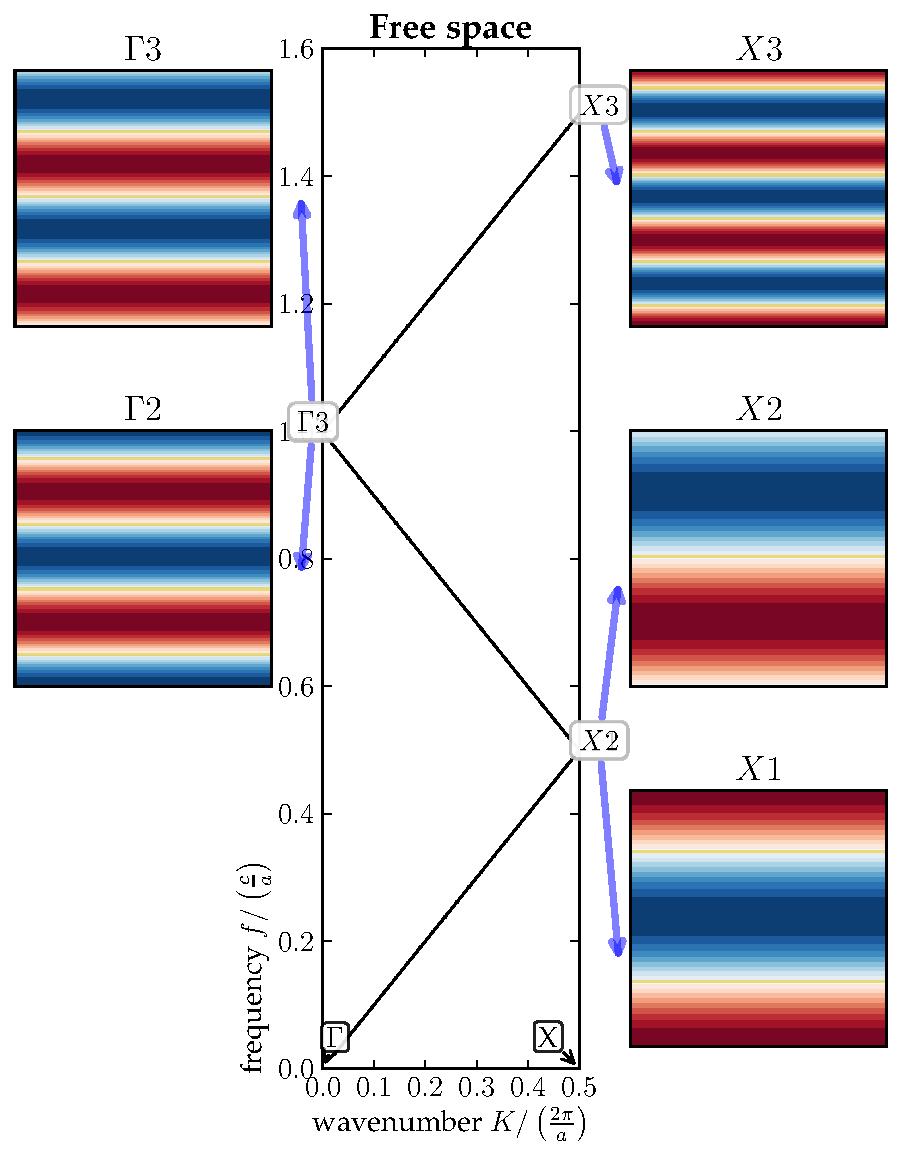
\includegraphics[width=8cm]{img/Slab_eps001_PWEM.pdf}
\textbf{b)}	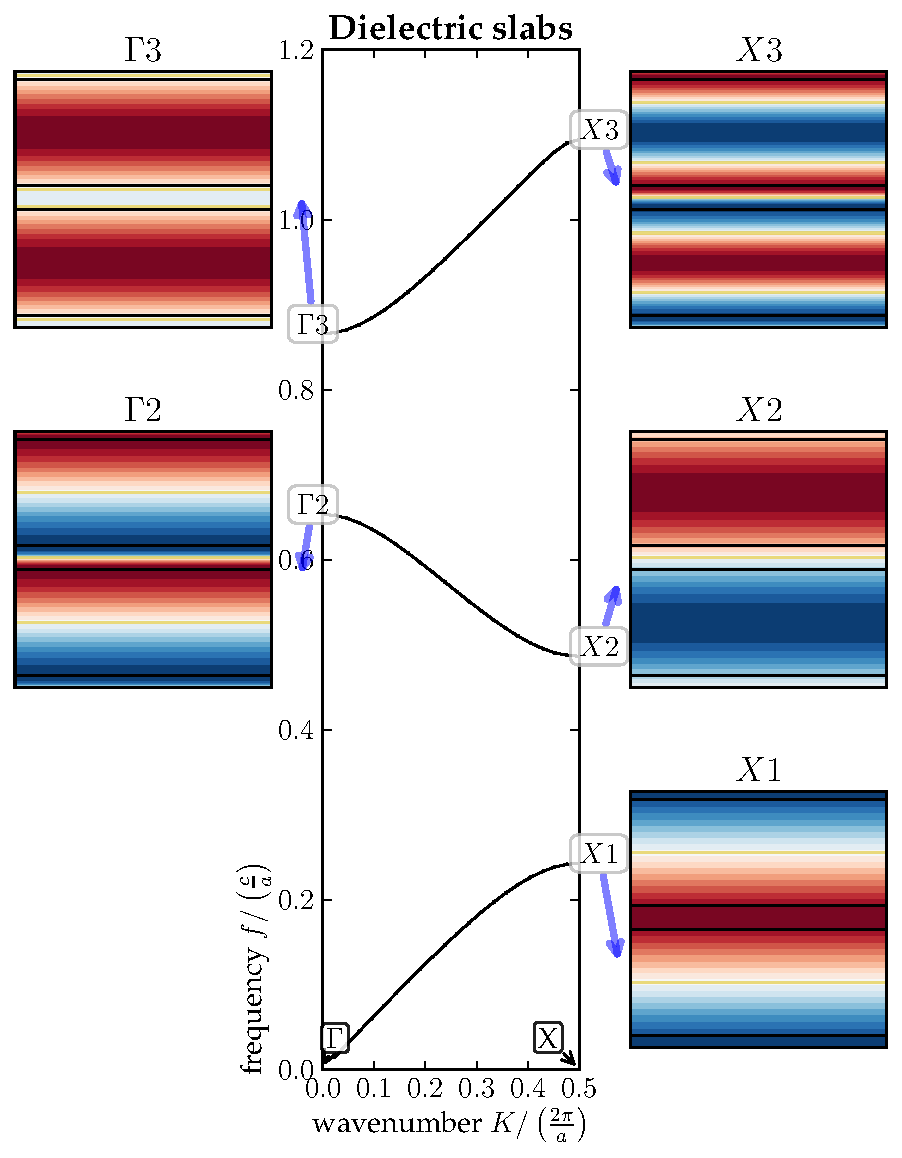
\includegraphics[width=8cm]{img/Slab_eps012_d15.pdf}
\end{figure}
% TODO draw and append axes+colorbar to the field distribution plots
% TODO visualise the permittivity, but how?

In Fig. \ref{fg_1dbd}a, we can see the folded dispersion curves for a plane wave propagating in vacuum, as already discussed above. 
%As predicted by the Bloch-Floquet theorem (\ref{eq_bloch}), the fields are periodic over each cell whenever the wavenumber $k$ touches the Brillouin zone boundary. 
To save space, we plot the  dispersion curves as \textit{folded}, but one can easily imagine how the curve unfolds into a straight light line. For any frequency $f$, there is a wavenumber $k$ corresponding to a propagating wave. 


The situation is different when we introduce periodic dielectric layers as in Fig. \ref{fg_1dbd}b. In the band structure, we observe allowed bands with \textit{band gaps} between them. At the frequencies in a bandgap, the wave can not propagate through the structure. The first photonic band ends when half the wavelength matches the cell spacing, i.e. when $2\pi / K= a/2$. The next band starts at the same wavenumber $K$, but the wave now has higher frequency because it is shifted by half its period so that it maximizes electric energy in air. For a 1-D photonic crystal, we can generally conclude that in order to move up on the frequency axis,
\begin{enumerate}
 \item{within each photonic band, one nodal plane per unit cell is added\footnote{In this paper, the mode plots show $2\times 2$ unit cells for clarity.},} 
 \item{within each photonic band gap, the wave shifts the most of electric field energy into lower-permittivity medium\footnote{Note that the band gaps do not have the same width on the frequency scale. For a certain thickness of the high-dielectric layer that corresponds to the Fabry-Pérot resonance, no frequency difference at all results from shifting the wave. In this case the band gap attains zero thickness, as is illustrated in Fig. \ref{fg_ebar_radiusscan}a for $r\approx20\,\upmu$m and $f\approx1.6$ THz. In other words, there may be a \textit{gap-less} transition between photonic bands.}, while the number of nodal planes remains constant. }
 \end{enumerate}

Such a shifting between waves at the lower and upper boundaries of the band gap is typical of classical \textit{Bragg} gaps that are responsible for the dispersion of the 1-D photonic crystal. 

\begin{figure} \caption{img/Slab\_eps001\_PWEM.pdf}  \centering 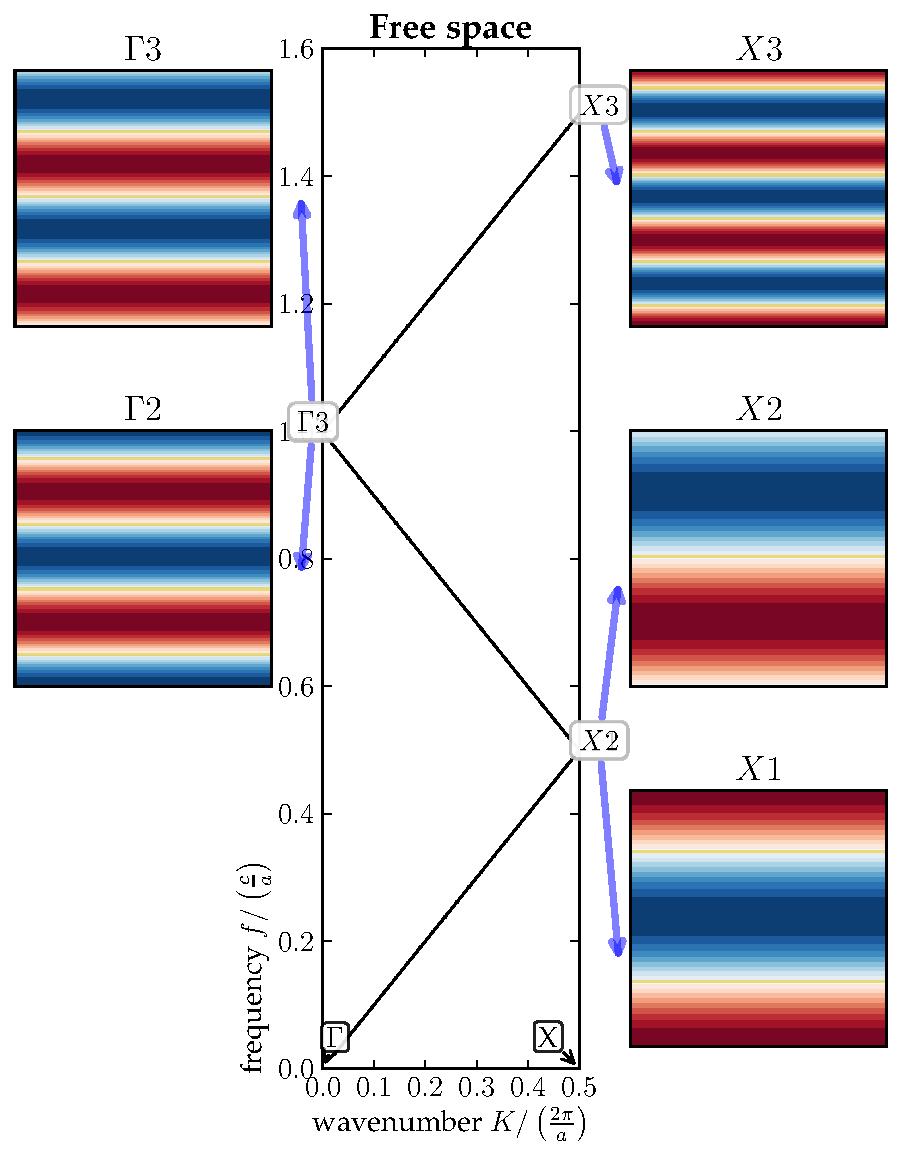
\includegraphics[width=10cm]{img/Slab_eps001_PWEM.pdf} \end{figure} \clearpage
\begin{figure} \caption{img/Slab\_eps012\_d15.pdf}  \centering 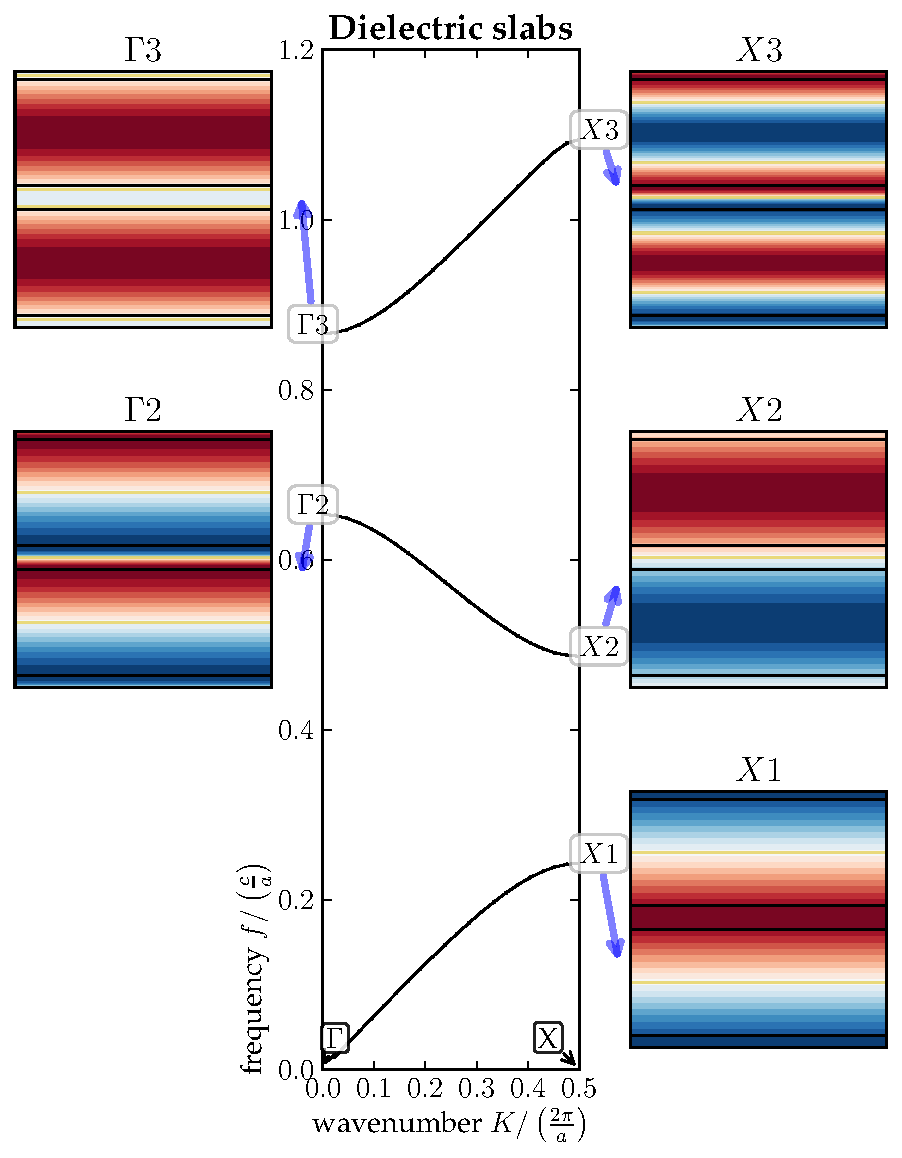
\includegraphics[width=10cm]{img/Slab_eps012_d15.pdf} \end{figure} \clearpage
%}}}

\subsection{Finite planar structure with defect mode} % references to ->
A defect-mode transmission peak of 1.5\% energy transmission appears in the band gap.
It can be tuned from 173 to 184 GHz by application of electric field (40 kV/cm) to the defect STO layer \cite{skoromets2013}.
%}}}

\section{Wire medium} % references to -> %{{{
\add{
We assume the medium is inductive $\quad \Rightarrow \quad  \varepsilon(f) = 1 - \frac{f_p^2}{f^2}$. 

\begin{itemize} \item{What is the plasma frequency $f_p$ for wires (with radius $r$ and spacing $a$)?} \end{itemize}

Pendry \textit{et al.} 1996: $\sqrt{\frac{c^2}{2\pi \, a^2 \, \log(\frac{a}{r})}}$

Maslovski \textit{et al.} 2003: $\sqrt{\frac{c^2}{2\pi \, a^2 \, \log\left(\frac{a^2}{4r (a-r)}\right)}}$

\begin{itemize} \item{How these models compare to the simulation?} \end{itemize}

\tiny{J. B. Pendry, A. J. Holden, W. J. Stewart, and I. Youngs, \textit{"Extremely low frequency plasmons in metallic meso structures,"} phys. rev. lett., vol. 76, pp. 4773–4776, 1996.  }\\
\tiny{Maslovski, S. I., Tretyakov, S. A. and Belov, P. A. (2002), \textit{Wire media with negative effective permittivity: A quasi-static model.} Microw. Opt. Technol. Lett., 35: 47–51. doi: 10.1002/mop.10512}
}

\begin{figure} \caption{img/XCylWire\_a100r4.pdf}  \centering 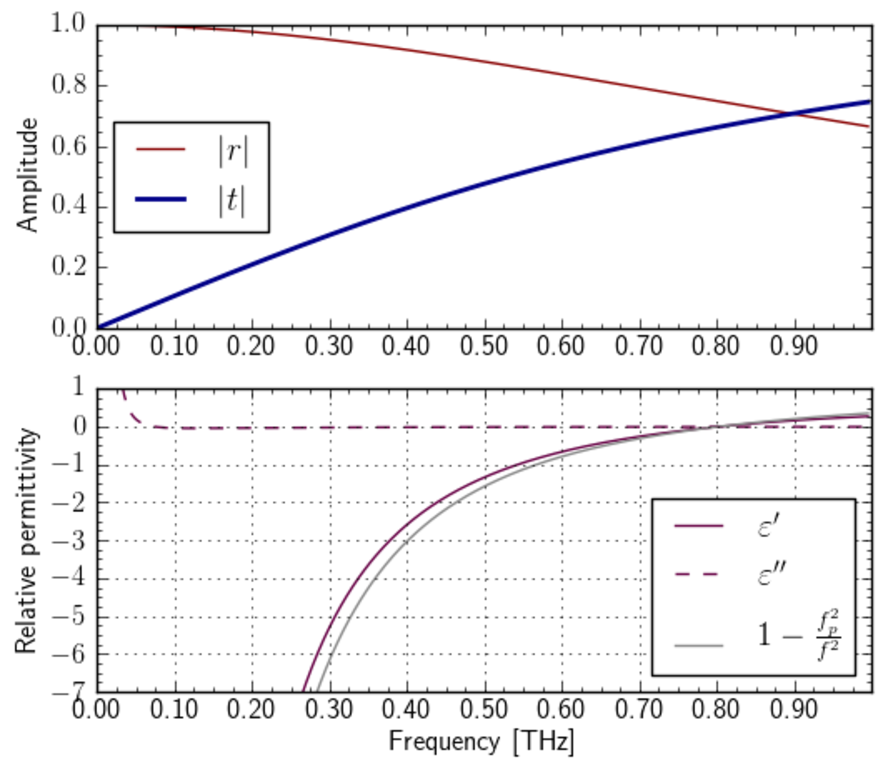
\includegraphics[width=10cm]{img/XCylWire_a100r4.pdf} \end{figure} \clearpage
\begin{figure} \caption{img/EWire\_plasmaF\_radiusscan.pdf}  \centering 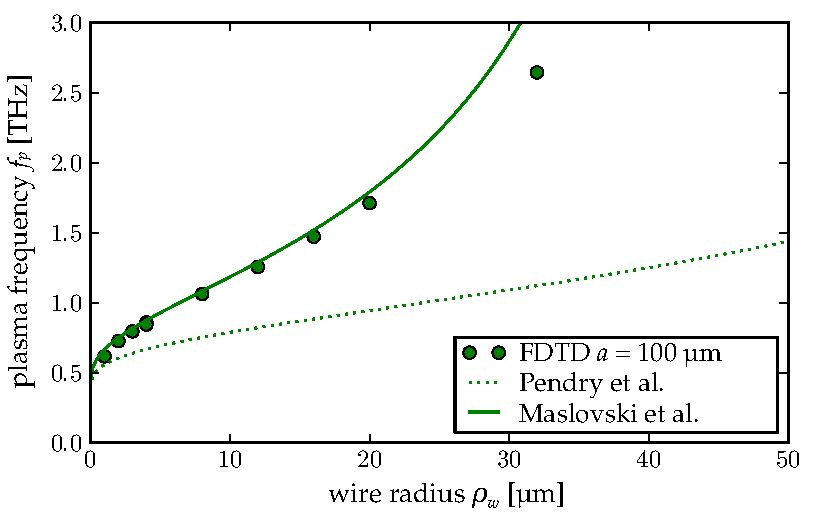
\includegraphics[width=10cm]{img/EWire_plasmaF_radiusscan.pdf} \end{figure} \clearpage
\begin{figure} \caption{img/EWire\_plasmaF\_spacingscan.pdf}  \centering 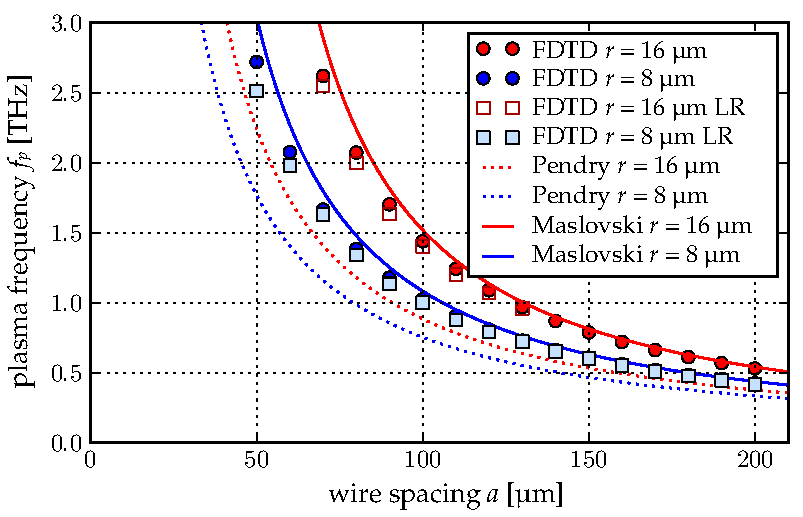
\includegraphics[width=10cm]{img/EWire_plasmaF_spacingscan.pdf} \end{figure} \clearpage
\begin{figure} \caption{img/EWire\_r03\_FDTDwide.pdf}  \centering 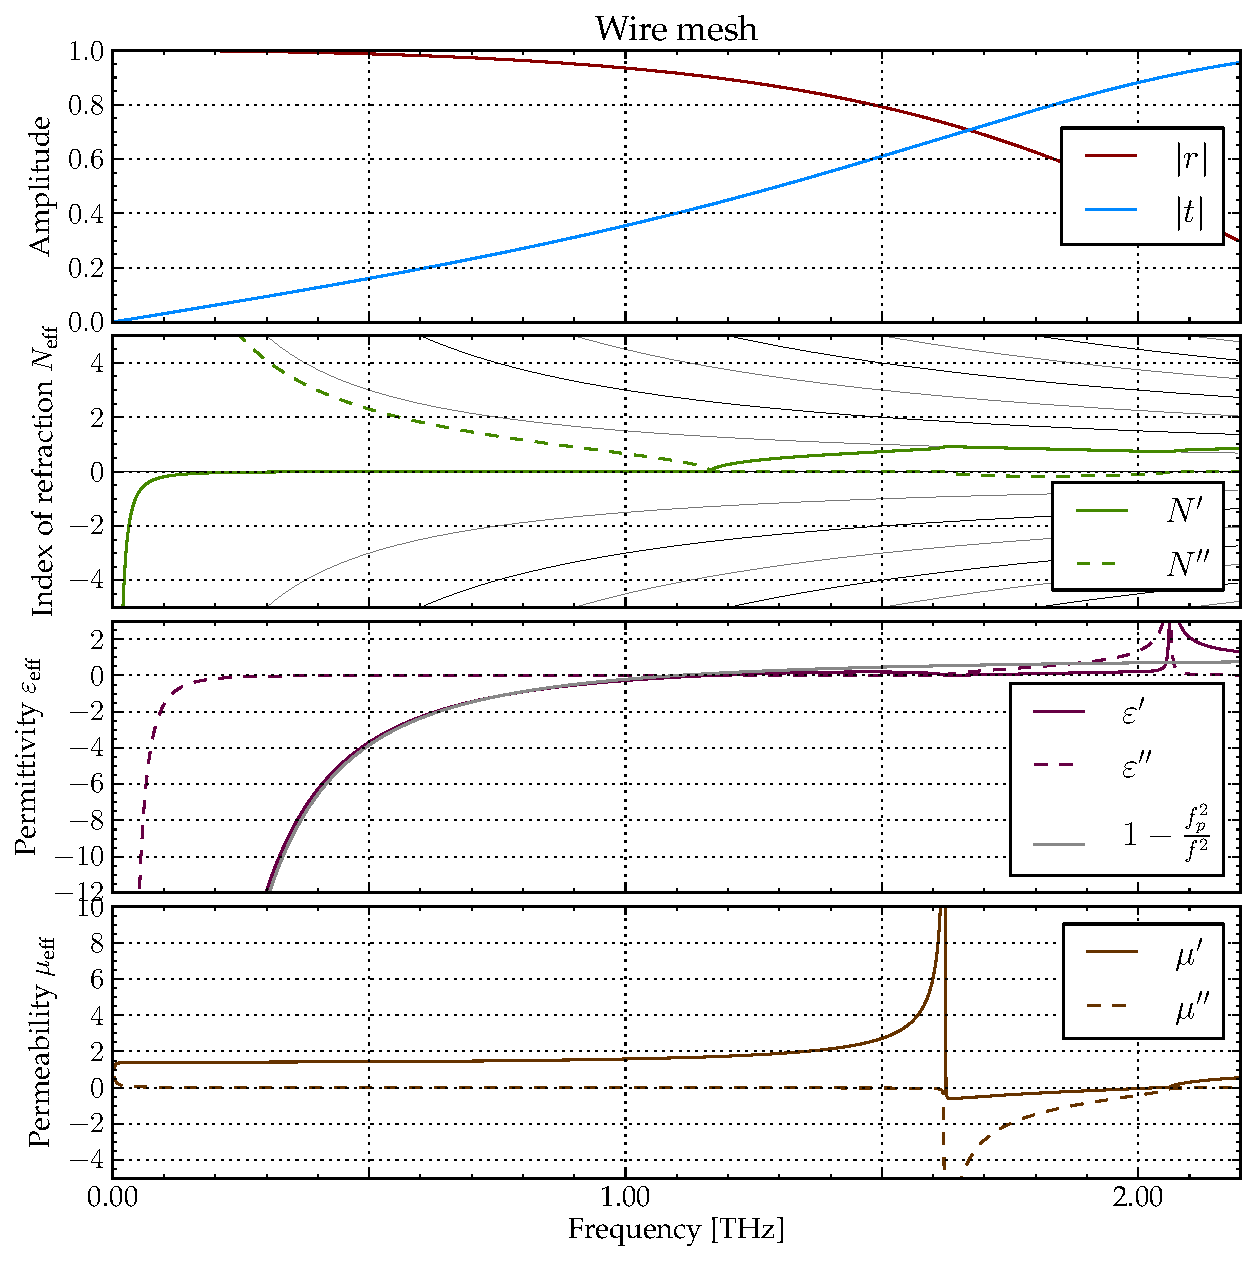
\includegraphics[width=10cm]{img/EWire_r03_FDTDwide.pdf} \end{figure} \clearpage
%}}}

\section{Metallic strips} % references to -> % note about plasmonic particles
\section{Metallic strip pair} % references to ->
\section{Split-ring resonator} % references to ->
\section{Dielectric sphere} % references to ->
%{{{
\begin{figure} \caption{img/Sphere\_eps100\_R25\_FDTD.pdf}  \centering 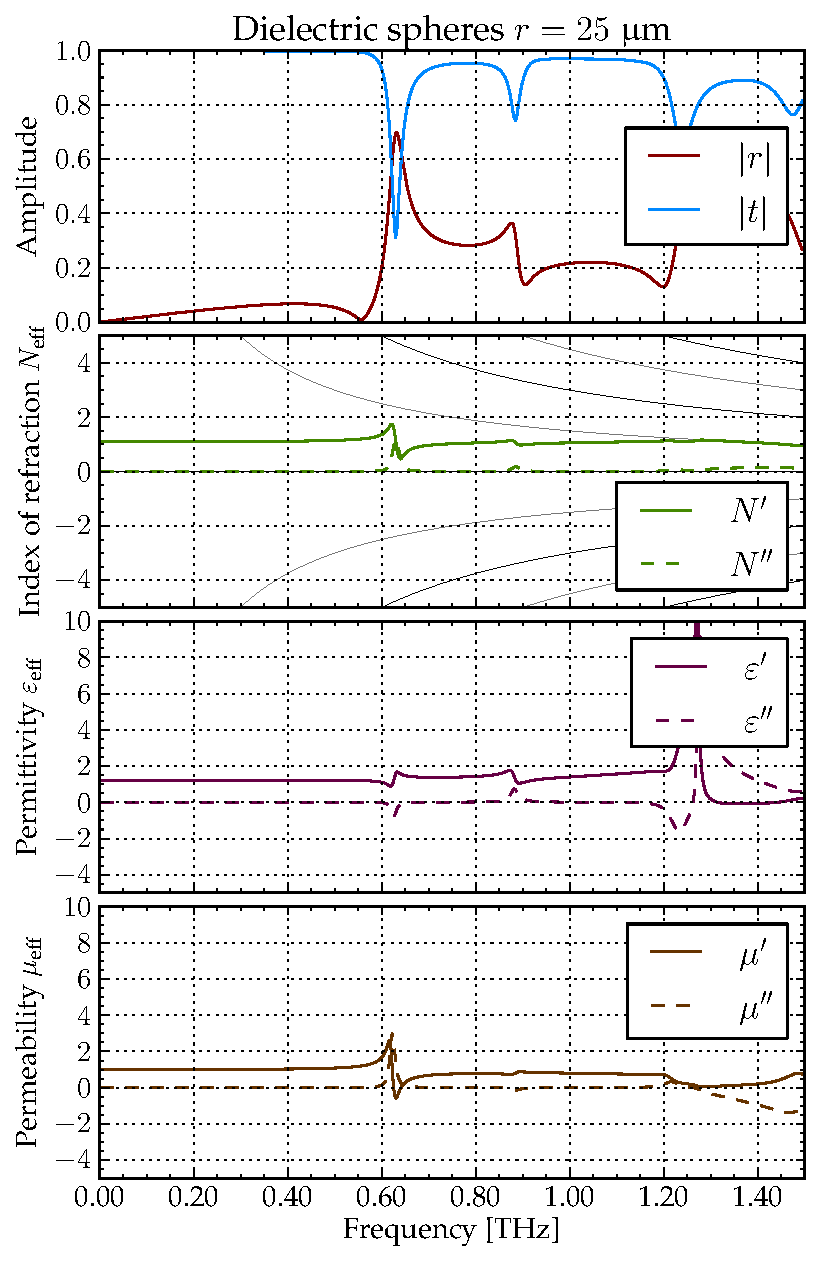
\includegraphics[width=10cm]{img/Sphere_eps100_R25_FDTD.pdf} \end{figure} \clearpage
\begin{figure} \caption{img/sphere\_Mie\_mode\_electric.pdf}  \centering 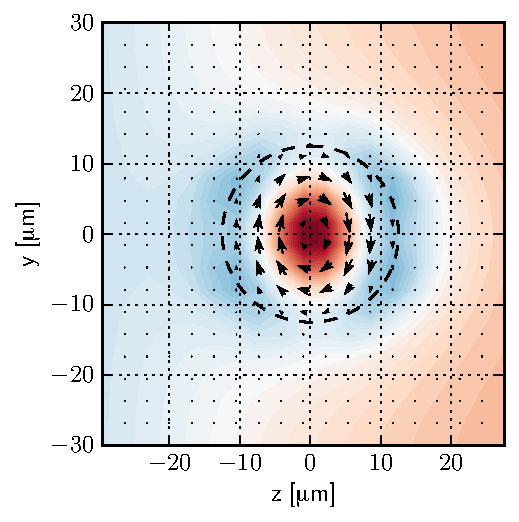
\includegraphics[width=10cm]{img/sphere_Mie_mode_electric.pdf} \end{figure} \clearpage
\begin{figure} \caption{img/sphere\_Mie\_mode\_magnetic.pdf}  \centering 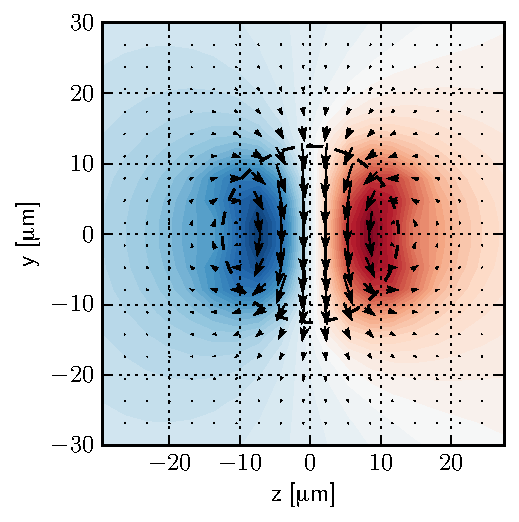
\includegraphics[width=10cm]{img/sphere_Mie_mode_magnetic.pdf} \end{figure} \clearpage
\begin{figure} \caption{img/Spheres\_FDTD\_experimentalConv.pdf}  \centering 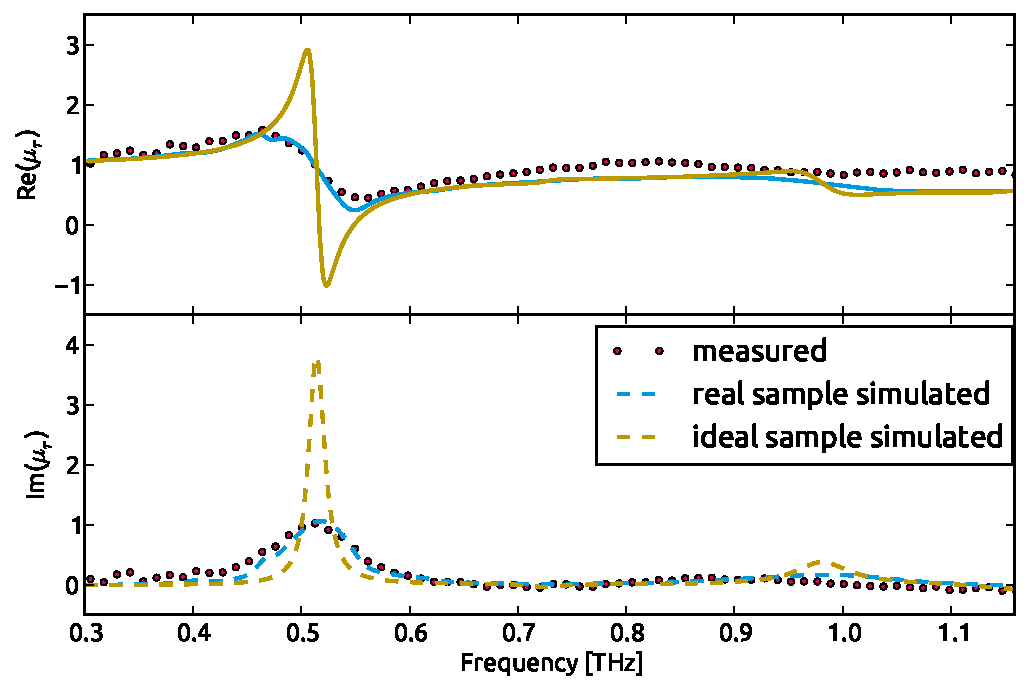
\includegraphics[width=10cm]{img/Spheres_FDTD_experimentalConv.pdf} \end{figure} \clearpage
%}}}
\section{SRRs and spheres in wire grid} % references to ->
%{{{
\begin{figure} \caption{img/SphereWire\_eps100\_R25\_FDTD.pdf}  \centering  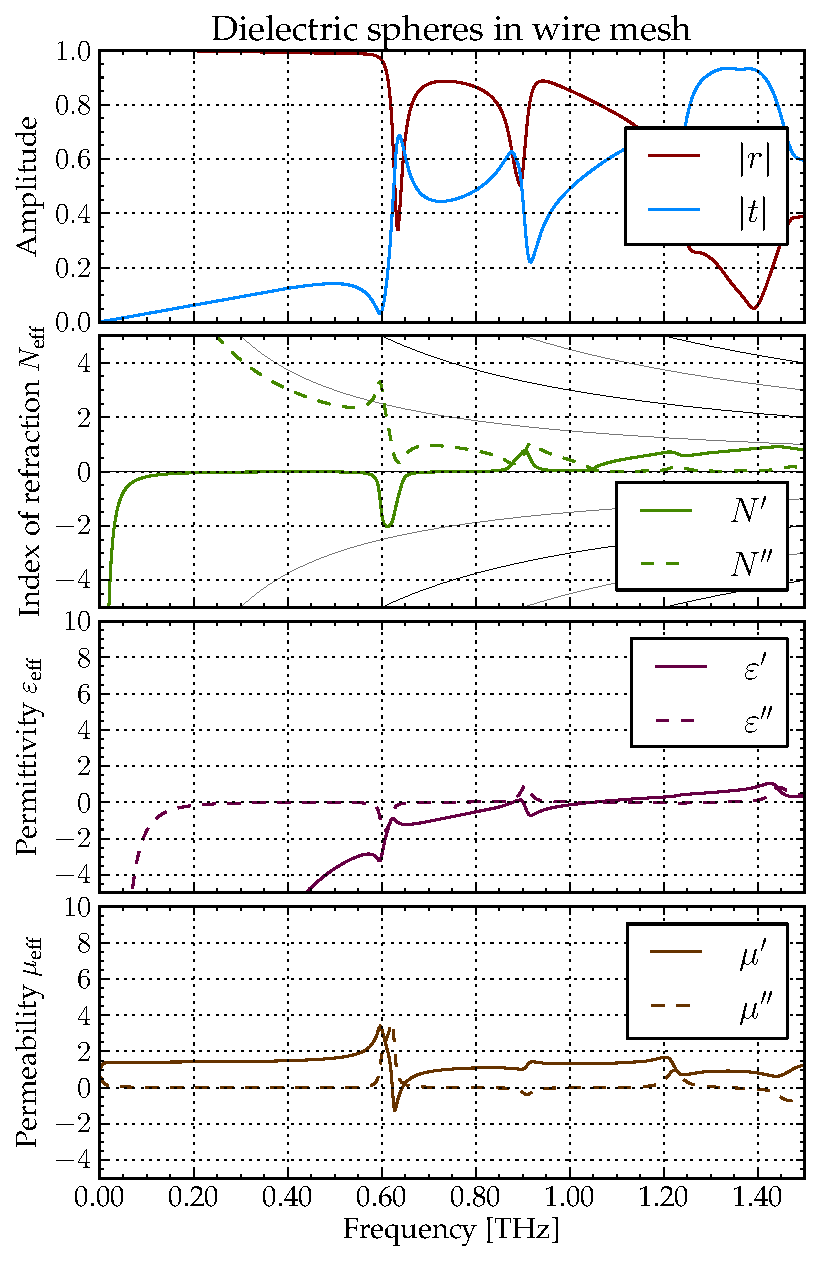
\includegraphics[width=10cm]{img/SphereWire_eps100_R25_FDTD.pdf} \end{figure} \clearpage
\begin{figure} \caption{SphereWire sketch}  \centering  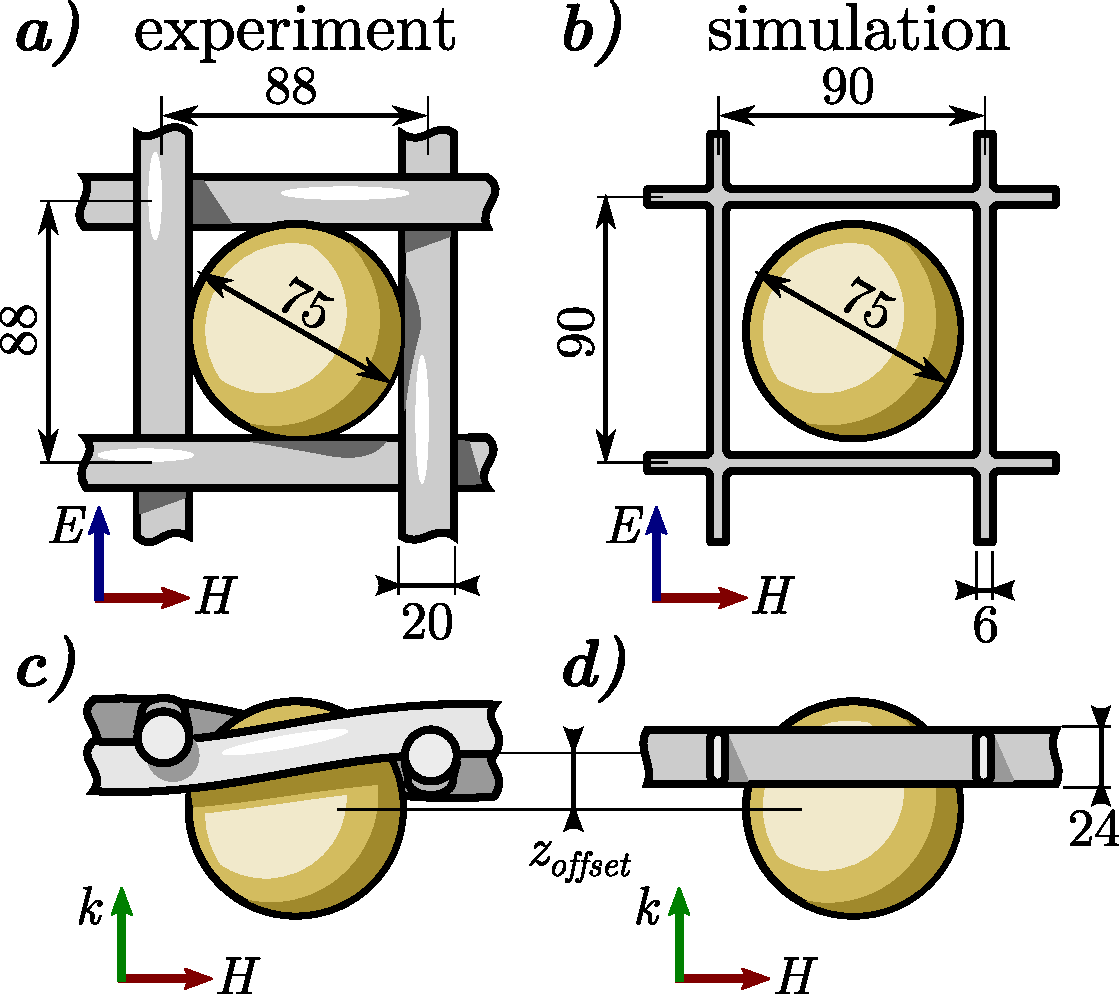
\includegraphics[width=10cm]{img/SphereWire_sketch.pdf} \end{figure} \clearpage
%}}}
\section{Dielectric rods parallel to magnetic field} % references to ->
%{{{
\begin{figure} \caption{img/HRods\_eps012\_R12\_PWEM.pdf}  \centering 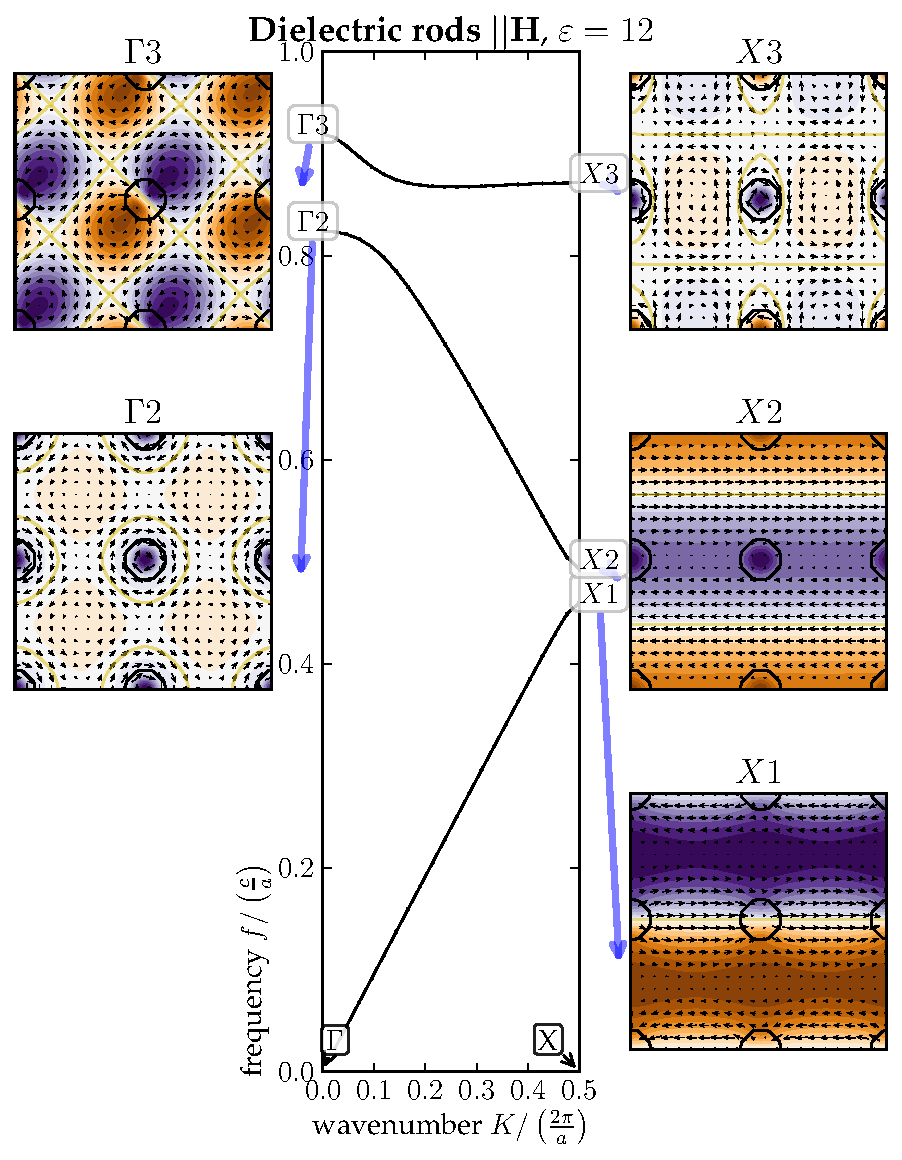
\includegraphics[width=10cm]{img/HRods_eps012_R12_PWEM.pdf} \end{figure} \clearpage
\begin{figure} \caption{img/HRods\_eps100\_R12\_FDTD.pdf}  \centering 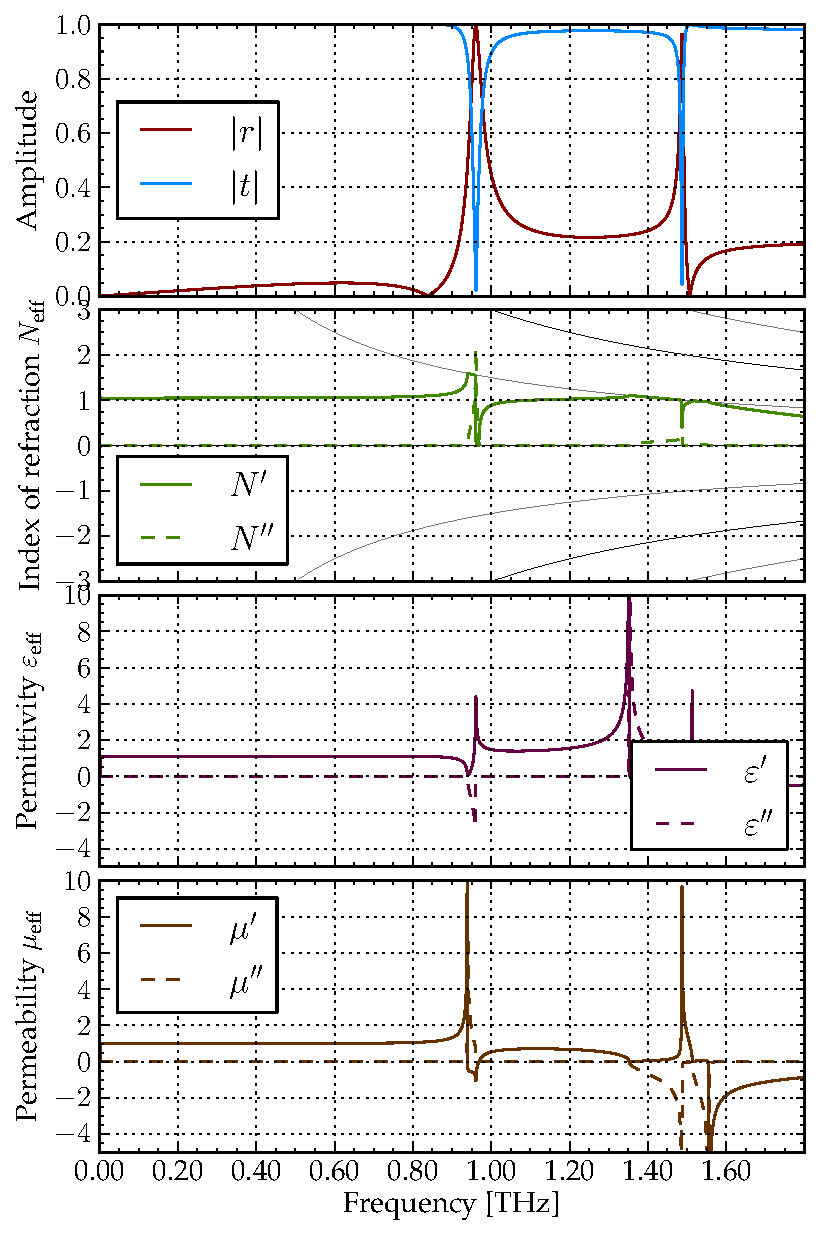
\includegraphics[width=10cm]{img/HRods_eps100_R12_FDTD.pdf} \end{figure} \clearpage
\begin{figure} \caption{img/HRods\_eps100\_R12\_PWEM.pdf}  \centering 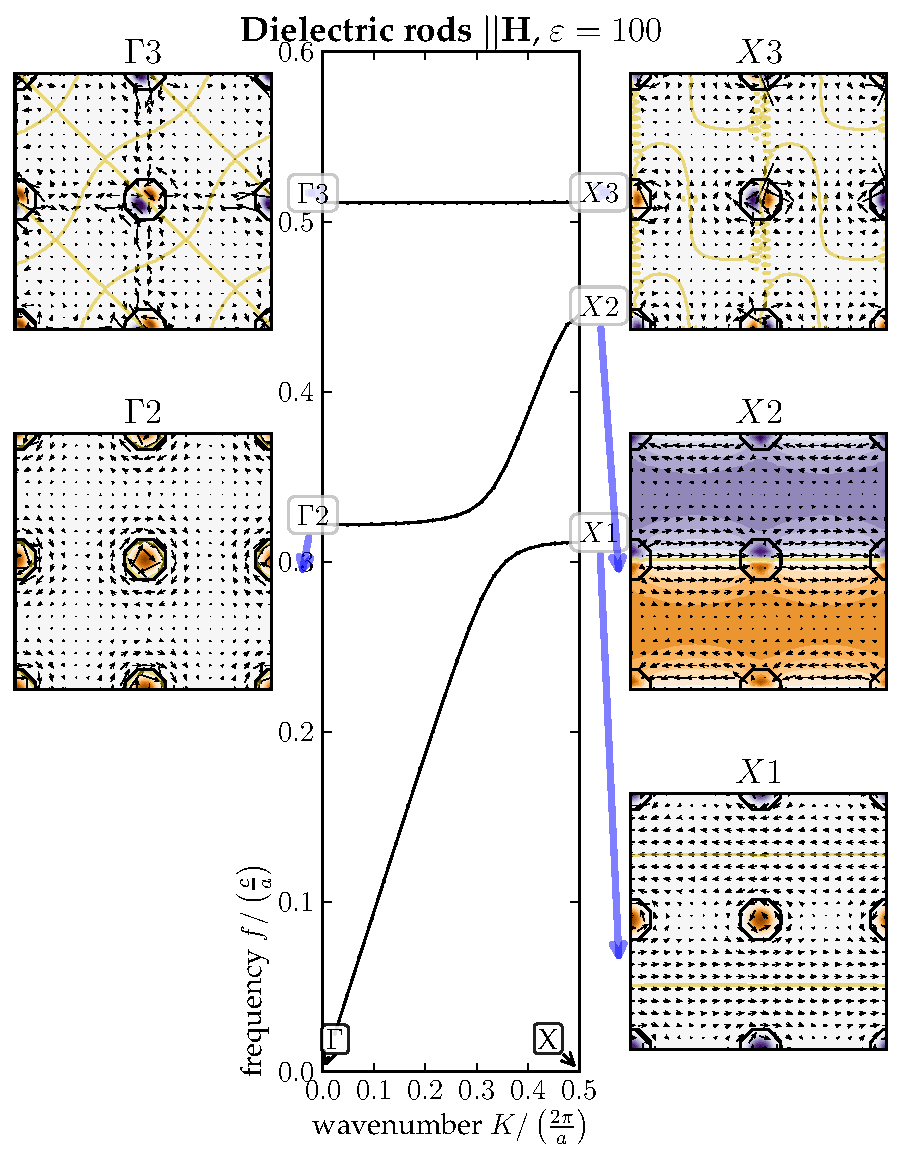
\includegraphics[width=10cm]{img/HRods_eps100_R12_PWEM.pdf} \end{figure} \clearpage
\begin{figure} \caption{img/HRods\_sketch.pdf}  \centering 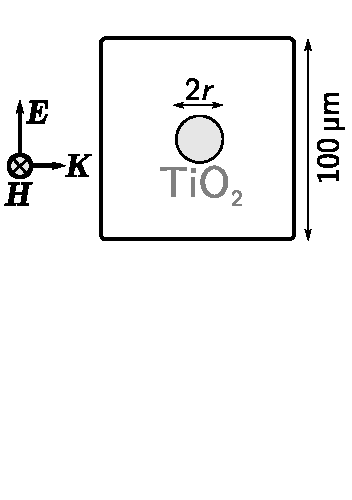
\includegraphics[width=10cm]{img/HRods_sketch.pdf} \end{figure} \clearpage
% todo? analytic Mie resonance frequency? -> OBrien&Pendry2002, szabos etc
\add{
Are there also different, non-Bragg, mechanisms that can create band gaps?


We would not indeed pose this question if its answer were negative. It is closely related to the \textit{internal resonances} based on non-propagating evanescent fields in the structure. The operation of all sorts of left-handed metamaterials  relies on these resonances. We conjecture such resonances may never occur in 1-D dielectric structures, so their study requires a simulation of a 2-D or 3-D structure.
% Todo elaborate the idea of nonBragg gap <-> nonradiative fields in structure <-> permittivity/permeability resonance
% Note that in 1-D dielectric PhC, all fields are propagating, none evanesecnt
% Big question: Can one approximate a metamaterial by ENG/DNG/MNG/DPS 1-D PhC??
\begin{figure}[ht] \caption{Dispersion curves for dielectric rods aligned parallel to magnetic field. The side plots show the shape of the fields in the $(x,z)$ plane, at the frequencies of the band edges. The magnetic field is plot as color map and the electric field is represented by vectors. The rod radius was chosen to 12 \% of the period. \textbf{a)} On the left, a relatively low permittivity $\varepsilon = 12$ places the magnetic resonance above the first Bragg band gap. \textbf{b)} For high permittivity dielectric $\varepsilon = 100$, the magnetic resonance forms the first band gap. } \label{fg_rodh} \centering 
\textbf{(a)}	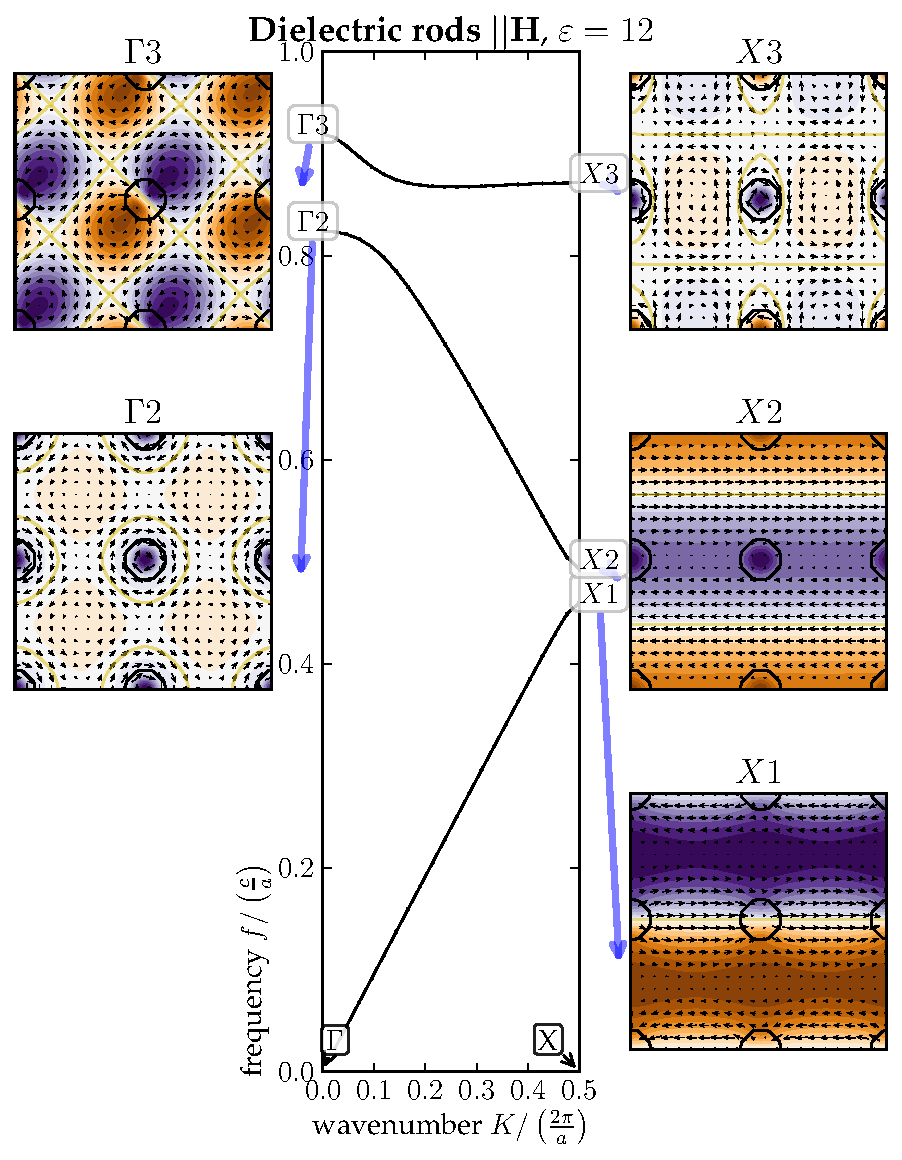
\includegraphics[width=8cm]{img/HRods_eps012_R12_PWEM.pdf}
\textbf{(b)}	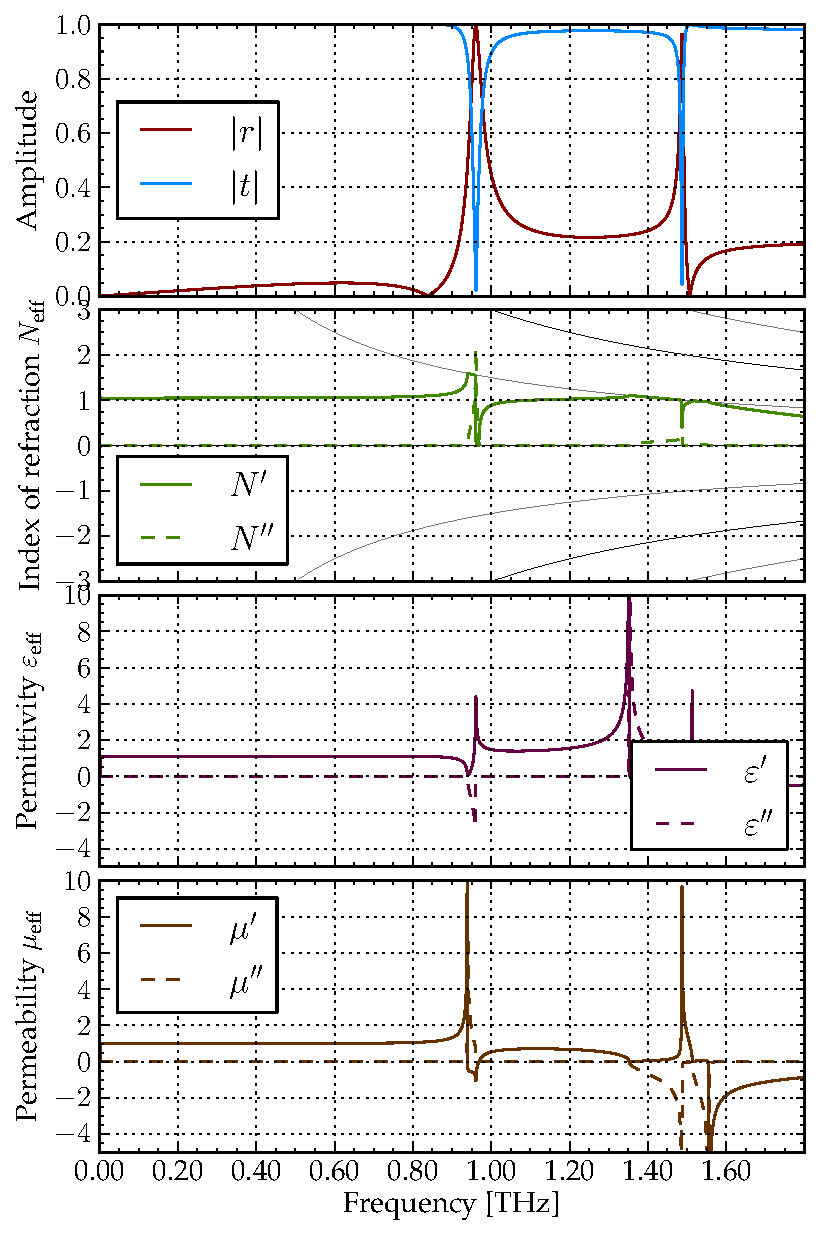
\includegraphics[width=8cm]{img/HRods_eps100_R12_FDTD.pdf}
\end{figure}

Probably the simplest example of such structures is a periodic array of high-permittivity dielectric rods, aligned parallel to the $y$-axis. (We use the convention that the structure is excited by a plane wave source with $\mathbf E || \mathbf x$, $\mathbf H || \mathbf y$ and the wave propagates along the $z$-axis). % dubious - the E, H have many directions in the unit cell; better  to write "TM"/"TE"? But this would confuse with nonperp incidence!
The inhomogeneity of the structure along the $x$-axis allows the electric field to circulate along the rod -- or, more precisely, the $\mathbf E$ field can now be decomposed into purely \textit{planar} part known from the previous section, and a purely \textit{circulating} part, that induces a magnetic flux near the rod axis. The circulating electric field is clearly visible on both plots in Fig. \ref{fg_rodh}, where all nonzero components of the fields ($H_y$, $E_x$ and $E_z$) are depicted. 

% discuss why this is not true: each lorentzian introduces delta mu -> so the low-frequency permeability of rod array should be > 1? Attracted to a magnet?
This new type of resonance is known as a \textit{magnetic Mie resonance}, \cite{obrien2002photonic, nemec2009tunable, yahiaoui2009broadband, yahiaoui2011tunable}. Unlike the Bragg gaps, it can be observed also in a single rod in free space. Being a function of the frequency of the incident wave, the magnetic dipole moment of the free-standing dielectric rod follows the characteristic Lorentzian shape of its \textit{resonance curve}. Below the resonance the magnetic dipole moment of the resonator goes to strongly positive values, while in a narrow region above the resonance it is strongly negative. How does this behaviour change if we arrange the rods in an infinite periodic array? 

%% TODO? Add the x, y, z, size scans of the ellipsoids%{{{
%> On 19 Mar 2014, at 15:57, <dominecf@fzu.cz>
%> wrote:
%>
%>> Dear Oleg and all,
%>> the frequency dependence of the Mie modes in an ellipsoid is
%>> nontrivial.
%>> Maybe some skilled mathematician could find the analytic expression,
%>> but I
%>> guess its evaluation would require a computer anyway. As an interesting
%>> numerical experiment with FDTD, I ran three scans over the X-, Y- and
%>> Z-
%>> semiaxes of a TiO2 ellipsoid, fixing the remaining semiaxes to 15 um.
%>> The
%>> ellipsoid's X-axis was oriented parallel to the electric field, the
%>> Z-axis
%>> pointed in the wave propagation direction.
%>>
%>> The results attached, best expressed by the dielectric loss spectra in
%>> bilogarithmic plot, show that the first (magnetic) mode is roughly
%>> proportional to X**(-0.4) and Z**(-0.4), while the dependence on the
%>> Y-size is even slower, similar to Y**(-0.2).
%>>
%>> The second Mie mode is more sensitive to the Z-size as Z**(-0.7), while
%>> the other sizes scale very slowly, X**(-0.15), Y**(-0.15).
%>>
%>> In all cases, the exponents of X, Y and Z~dependencies should sum up to
%>> -1, which is the obvious rule for the frequency dependence when all
%>> axes
%>> are scaled simultaneously!
%>>
%>> Note that these estimated exponents are roughly valid only near the
%>> spherical shape, ie. when X~Y~Z. As a matter of fact, the tuning curves
%>> are not straight in the log-log plots. Naturally when one ellipsoid
%>> dimension is much lower than the other two, its role becomes more
%>> pronounced.
%>>
%>> Now we are coming to the big conclusion: Near the spherical shape, the
%>> difference of exponential slope between X- and Y- elongation is
%>> (0.4-0.2)=0.2. Therefore, (15./12.)**(0.4-0.2) gives a reasonable
%>> factor
%>> of 1.0456 difference for the resonant frequencies of the magnetic mode.%}}}

The results from a PWEM computation are plot in Fig. \ref{fg_rodh}. To obtain comparable dispersion curves in Fig. \ref{fg_rodh_fdtd}, we employed the FDTD simulation and the effective parameter retrieval described above. The main differences are that in Fig. \ref{fg_rodh_fdtd} we plot the frequency $f$ on the horizontal axis and we also use the effective index of refraction $N_{\text{eff}} := K\cdot \frac{c}{2\pi\,f}$ instead of the wavenumber $K$. One advantage of this representation is that $N_{\text{eff}}$ should be compliant with the Kramers-Kronig relations. This criterion always gives \textit{only one} correct solution on how to unfold $K$ to obtain realistic $N_{\text{eff}}$. 
In the simulation, the rod spacing (or, lattice constant) $a$ was 100 $\upmu$m, so the normalised frequency unit is $c/a = 3$ THz. The frequency range from 0 to 1.8 THz was therefore chosen the same as in Fig. \ref{fg_rodh}b. 
Note the first resonance shows pronounced resonant shape in the plot of permeability, which is typical of magnetic Mie resonances. In a very narrow region 960-970 GHz, the permeability $\mu_{\text{eff}}$ is real and negative. 
Apart from $N_{\text{eff}}$, the FDTD computation gives also the effective wave impedance $Z_{\text{eff}}$, which is a complementary information we need to compute the effective permittivity $\varepsilon_{\text{eff}}$ and the effective permeability $\mu_{\text{eff}}$:

\begin{equation} \varepsilon_{\text{eff}} = N_{\text{eff}}/Z_{\text{eff}}, \quad\quad\quad\quad \mu_{\text{eff}} = N_{\text{eff}}\cdot Z_{\text{eff}}.
\label{eq_epsmu}\end{equation}

\begin{figure}[ht]  \caption{Effective parameters of an array of dielectric rods $||\mathbf H$ with same parameters as in Fig. \ref{fg_rodh}b (i.e. radius of  12 \% of the period and permittivity $\varepsilon = 100$). Complex reflection $r$ and transmission $t$ spectra allow to compute the effective index of refraction, impedance (not shown), permittivity and permeability. Thin grey lines indicate the Brillouin zone boundaries.}
\label{fg_rodh_fdtd} \centering 
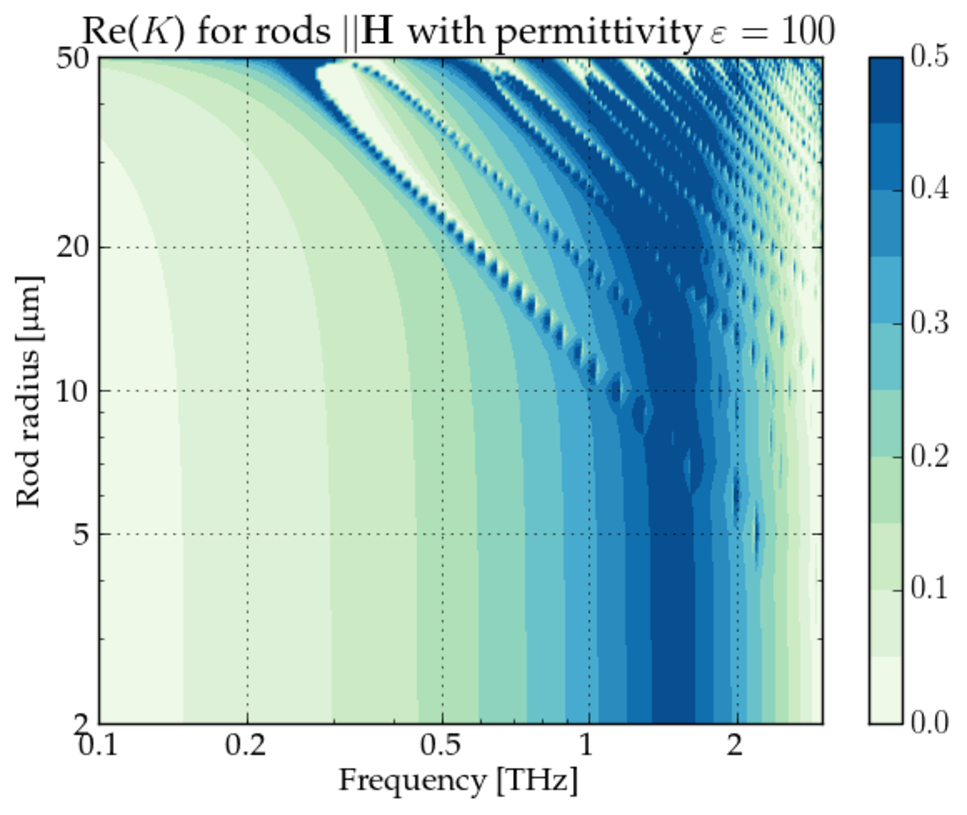
\includegraphics[width=8cm]{img/HRods_eps100_radiusscan.pdf}
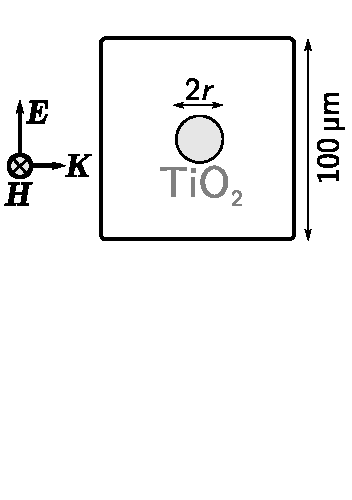
\includegraphics[width=4.5cm]{img/HRods_sketch.pdf}
\end{figure}

Other Mie resonances are located at higher frequencies. As a general rule for similar structures, the odd-numbered resonances have magnetic dipole moment (along the rod axis), whereas the even-numbered resonances have electric dipole moment (perpendicular to the rod axis). The reason is that electric dipole moments in odd resonances are suppressed due to antisymmetric shape of the mode; naturally the same holds for the magnetic moments in the even resonances.

The frequency of the Mie resonances is not significantly influenced by the photonic bands. Therefore, in order to understand the resulting band structure and its dependence on parameters, one has to disentangle which band gaps are due to Bragg reflection and which correspond to magnetic or electric Mie resonances. This is much easier knowing the spectra of $\varepsilon_{\text{eff}}$ and $\mu_{\text{eff}}$, as provided by FDTD in Fig. \ref{fg_rodh_fdtd}.
\begin{figure}[ht] \caption{The spectra of the wavenumber $K$ for different rod radii and two different rod permittivities. The wavenumber plot is folded so it ranges from 0 to 0.5, where $K\approx 0$ and $K\approx 0.5$ correspond to band gaps. \textbf{a)} Medium-permittivity rods with $\varepsilon = 12$, \textbf{b)} high-permittivity rods with $\varepsilon = 100$.  } \label{fg_hbar_radiusscan} \centering 
\textbf{a)}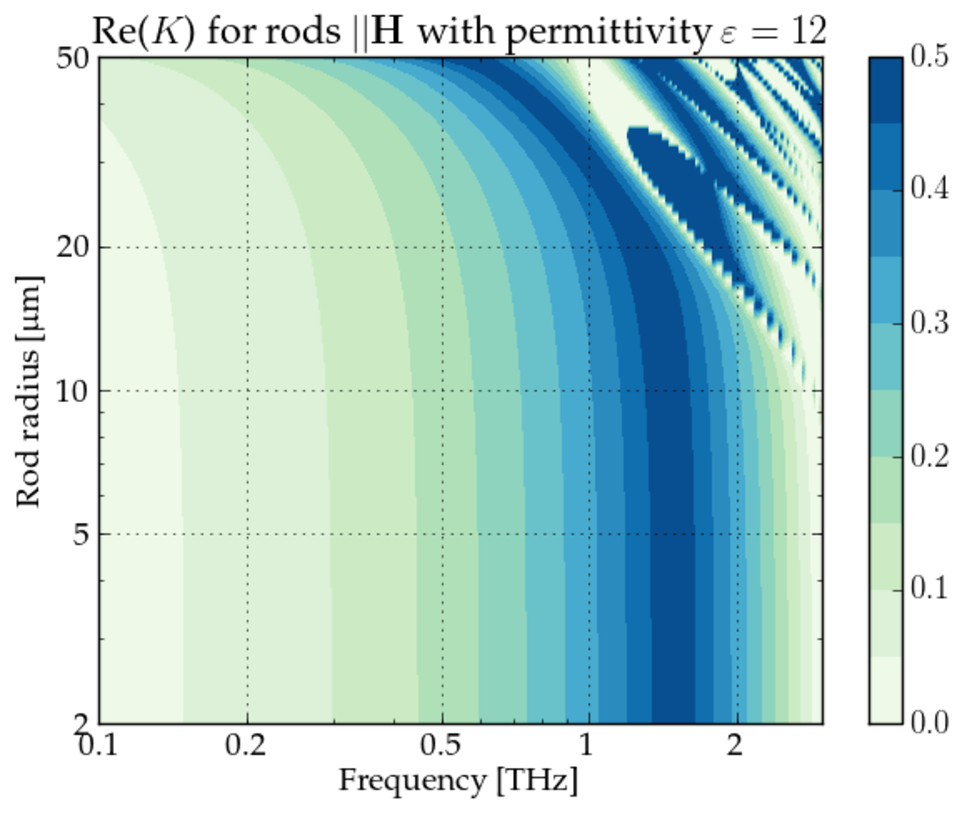
\includegraphics[width=8cm]{img/HRods_eps012_radiusscan.pdf}
\textbf{b)}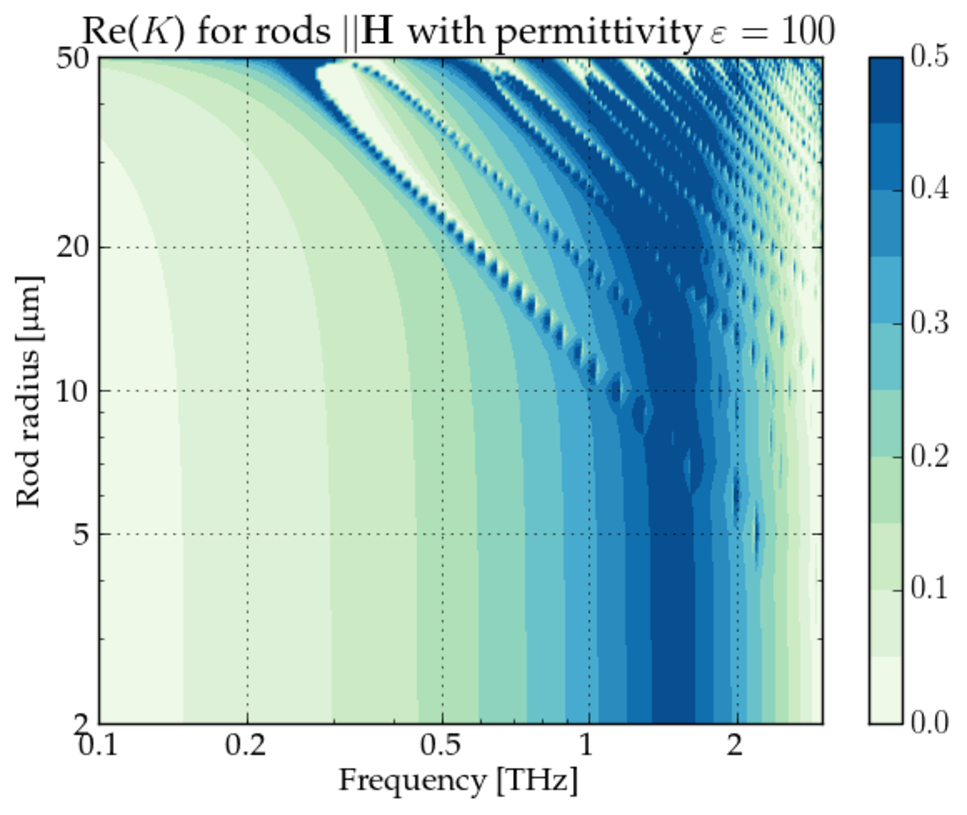
\includegraphics[width=8cm]{img/HRods_eps100_radiusscan.pdf}
\end{figure}

The photonic crystals composed of square lattice of dielectric rods have been examinated thoroughly since early 90s \cite{plihal1991two, pendry1992_transfer_matrix}. The permittivity of the constituent materials was rather low, corresponding to the optical or near-infrared frequencies, where the suitable materials usually have permittivity $\varepsilon < 12$. By parametric scans we could prove that for rod permittivity below 60 or even 80, the individual resonance is always located at higher frequency than the Bragg gap. Little, if any, attention was therefore paid to different nature of the higher resonances and most publications focused on properties and applications of the Bragg band gap.

The situation is different in the terahertz range, as the lattice of the crystalline solids often exhibits optical phonons at frequencies between 5 and 20 THz. The permittivity of many materials turns out to be much higher for frequencies below these resonances. This enables to conceive structures composed e.g. of titanium dioxide \cite{baumard1977_epsilon_TiO2} with $\varepsilon^{\text{THz}} \approx 92$ or of ferroelectrics with $\varepsilon^{\text{THz}}$ even orders of magnitude higher \cite{skoromets2011tuning}. The price to be paid for this advantage in the THz range are the relatively high losses caused by the lattice vibrations.
}

\begin{figure}[ht] \caption{Behaviour of the rods $||\mathbf E$, with permittivity $\varepsilon = 100$ and radius $r=11\;\upmu$m.\\
\textbf{a)} Band diagram and modes from PWEM. 
\textbf{b)} The effective parameters computed using FDTD confirm the previous results.  } \label{fg_erod_radius11} \centering 
\textbf{a)}	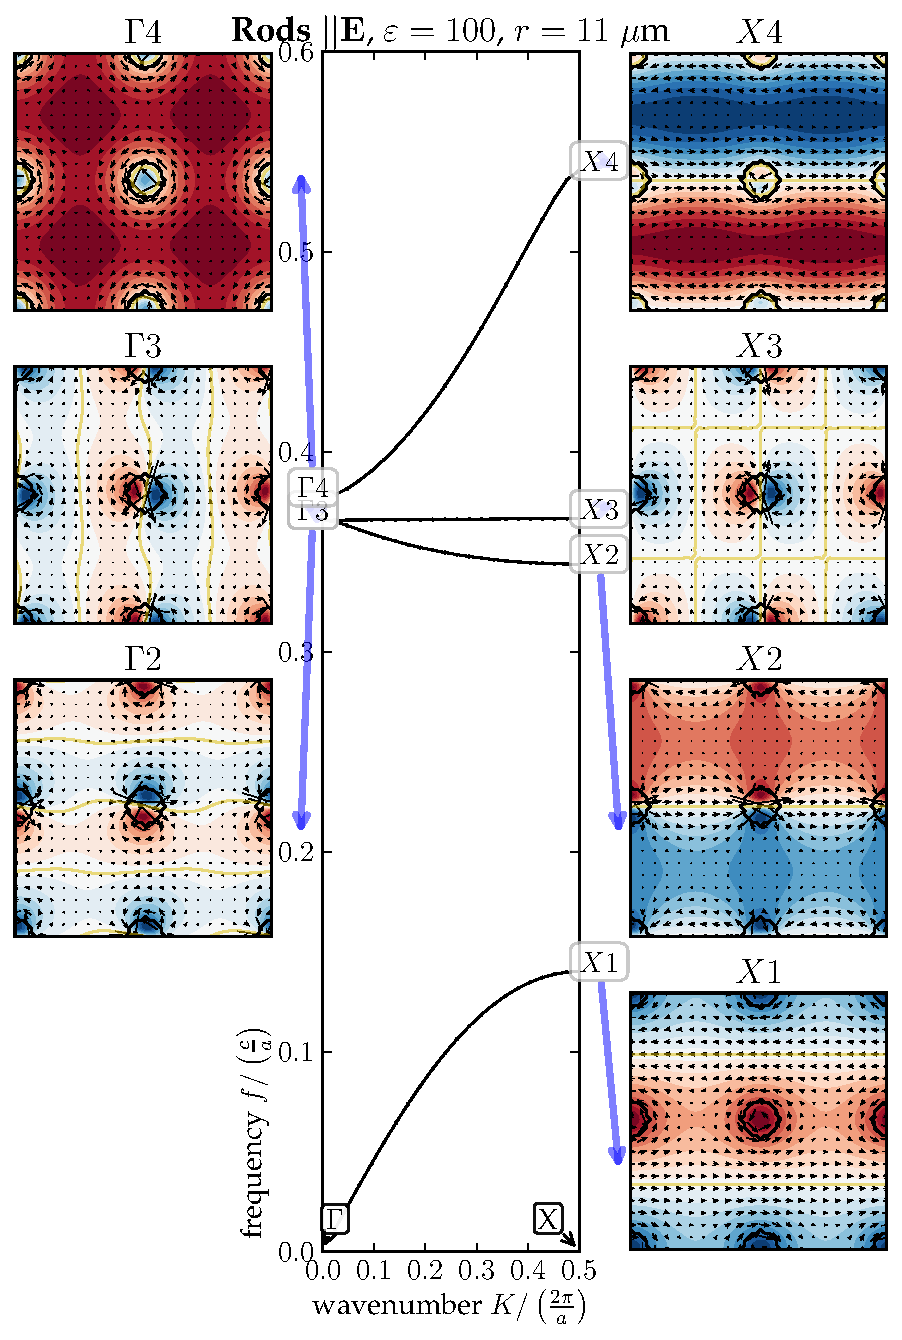
\includegraphics[width=8.5cm]{img/ERods_eps100_R11_PWEM.pdf}
\textbf{b)}	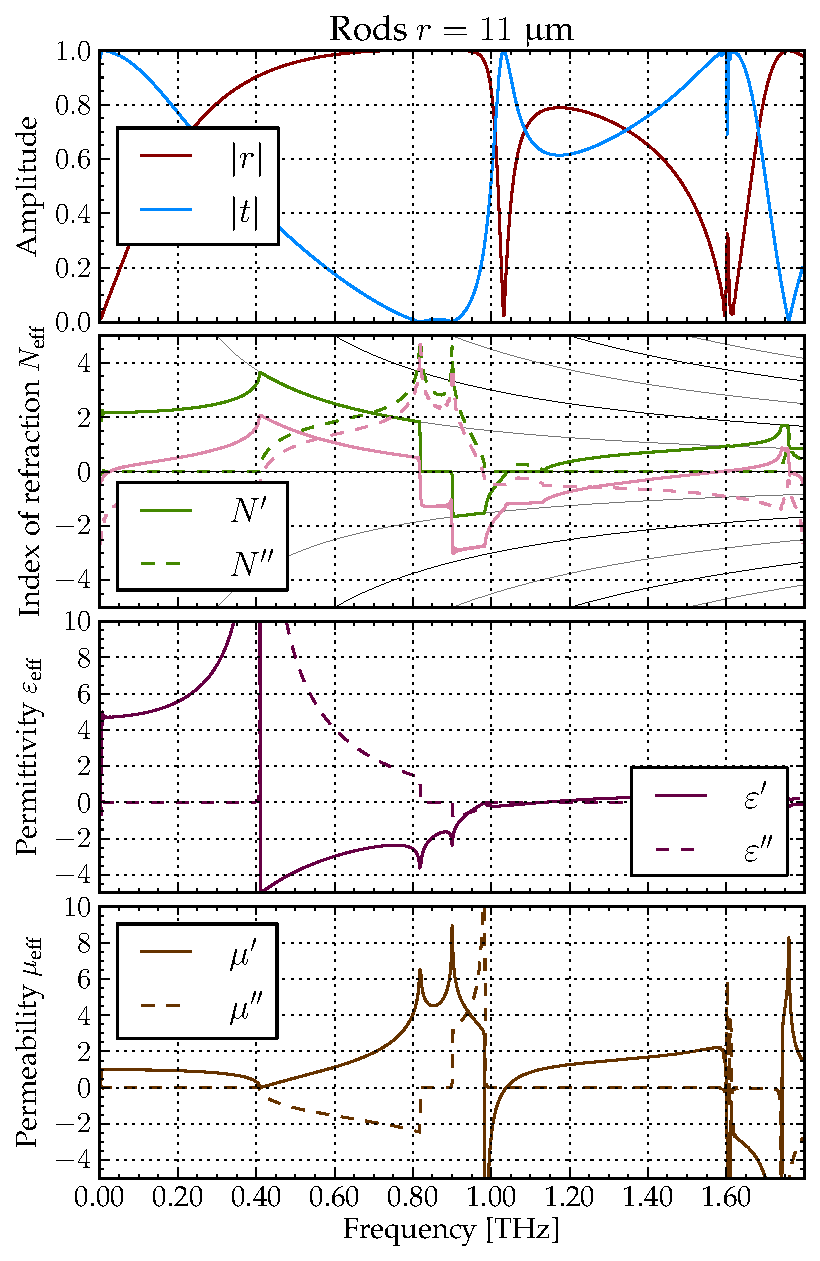
\includegraphics[width=8.0cm]{img/ERods_eps100_11um_FDTD.pdf}
\end{figure}

%}}}
\section{STO bar TODO} % references to ->
%{{{
\begin{figure} \caption{img/STOBar\_photo\_narrow.pdf}  \centering 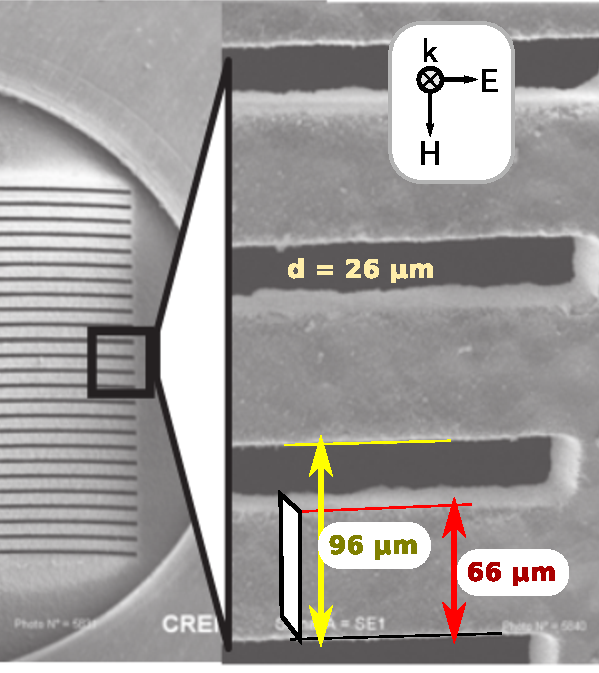
\includegraphics[width=10cm]{img/STOBar_photo_narrow.pdf} \end{figure} \clearpage
\begin{figure} \caption{img/STOBar\_photo.pdf}  \centering 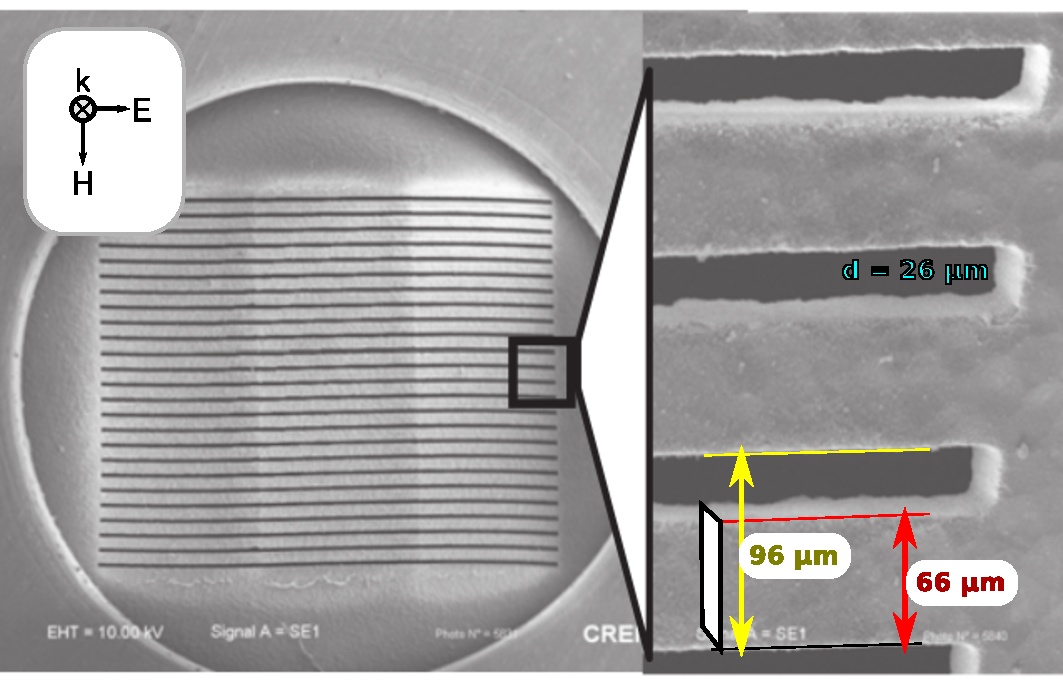
\includegraphics[width=10cm]{img/STOBar_photo.pdf} \end{figure} \clearpage
\begin{figure} \caption{img/STObar\_rt.pdf}  \centering 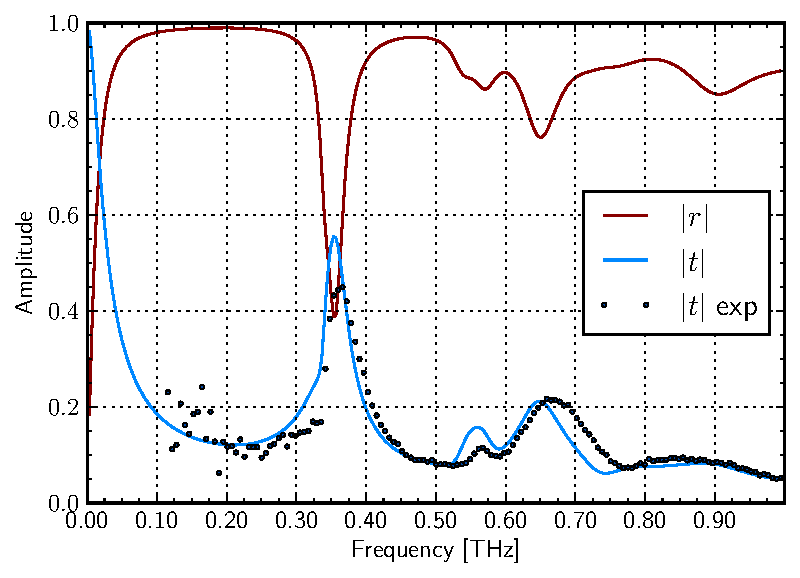
\includegraphics[width=10cm]{img/STObar_rt.pdf} \end{figure} \clearpage
%}}}
\section{Dielectric rods parallel to electric field} % references to ->
%{{{
% TODO refereence  also to \cite{valdivia2012} and \cite{shi2007}
\begin{figure} \caption{img/EBars\_STO\_sketch.pdf}  \centering 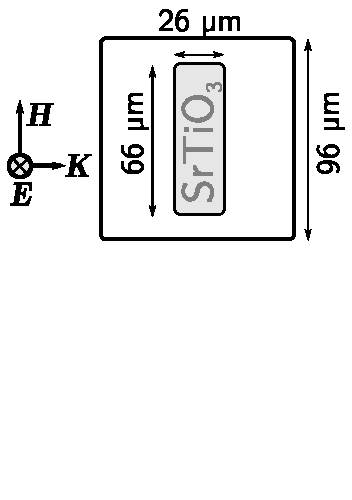
\includegraphics[width=10cm]{img/EBars_STO_sketch.pdf} \end{figure} \clearpage

\begin{figure} \caption{img/ERods\_1st\_and\_2nd\_Mie\_resonance.pdf}  \centering 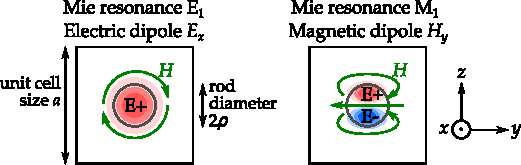
\includegraphics[width=10cm]{img/ERods_1st_and_2nd_Mie_resonance.pdf} \end{figure} \clearpage

\begin{figure} \caption{img/ERods\_eps100\_double\_a100a080\_FDTD.pdf}  \centering 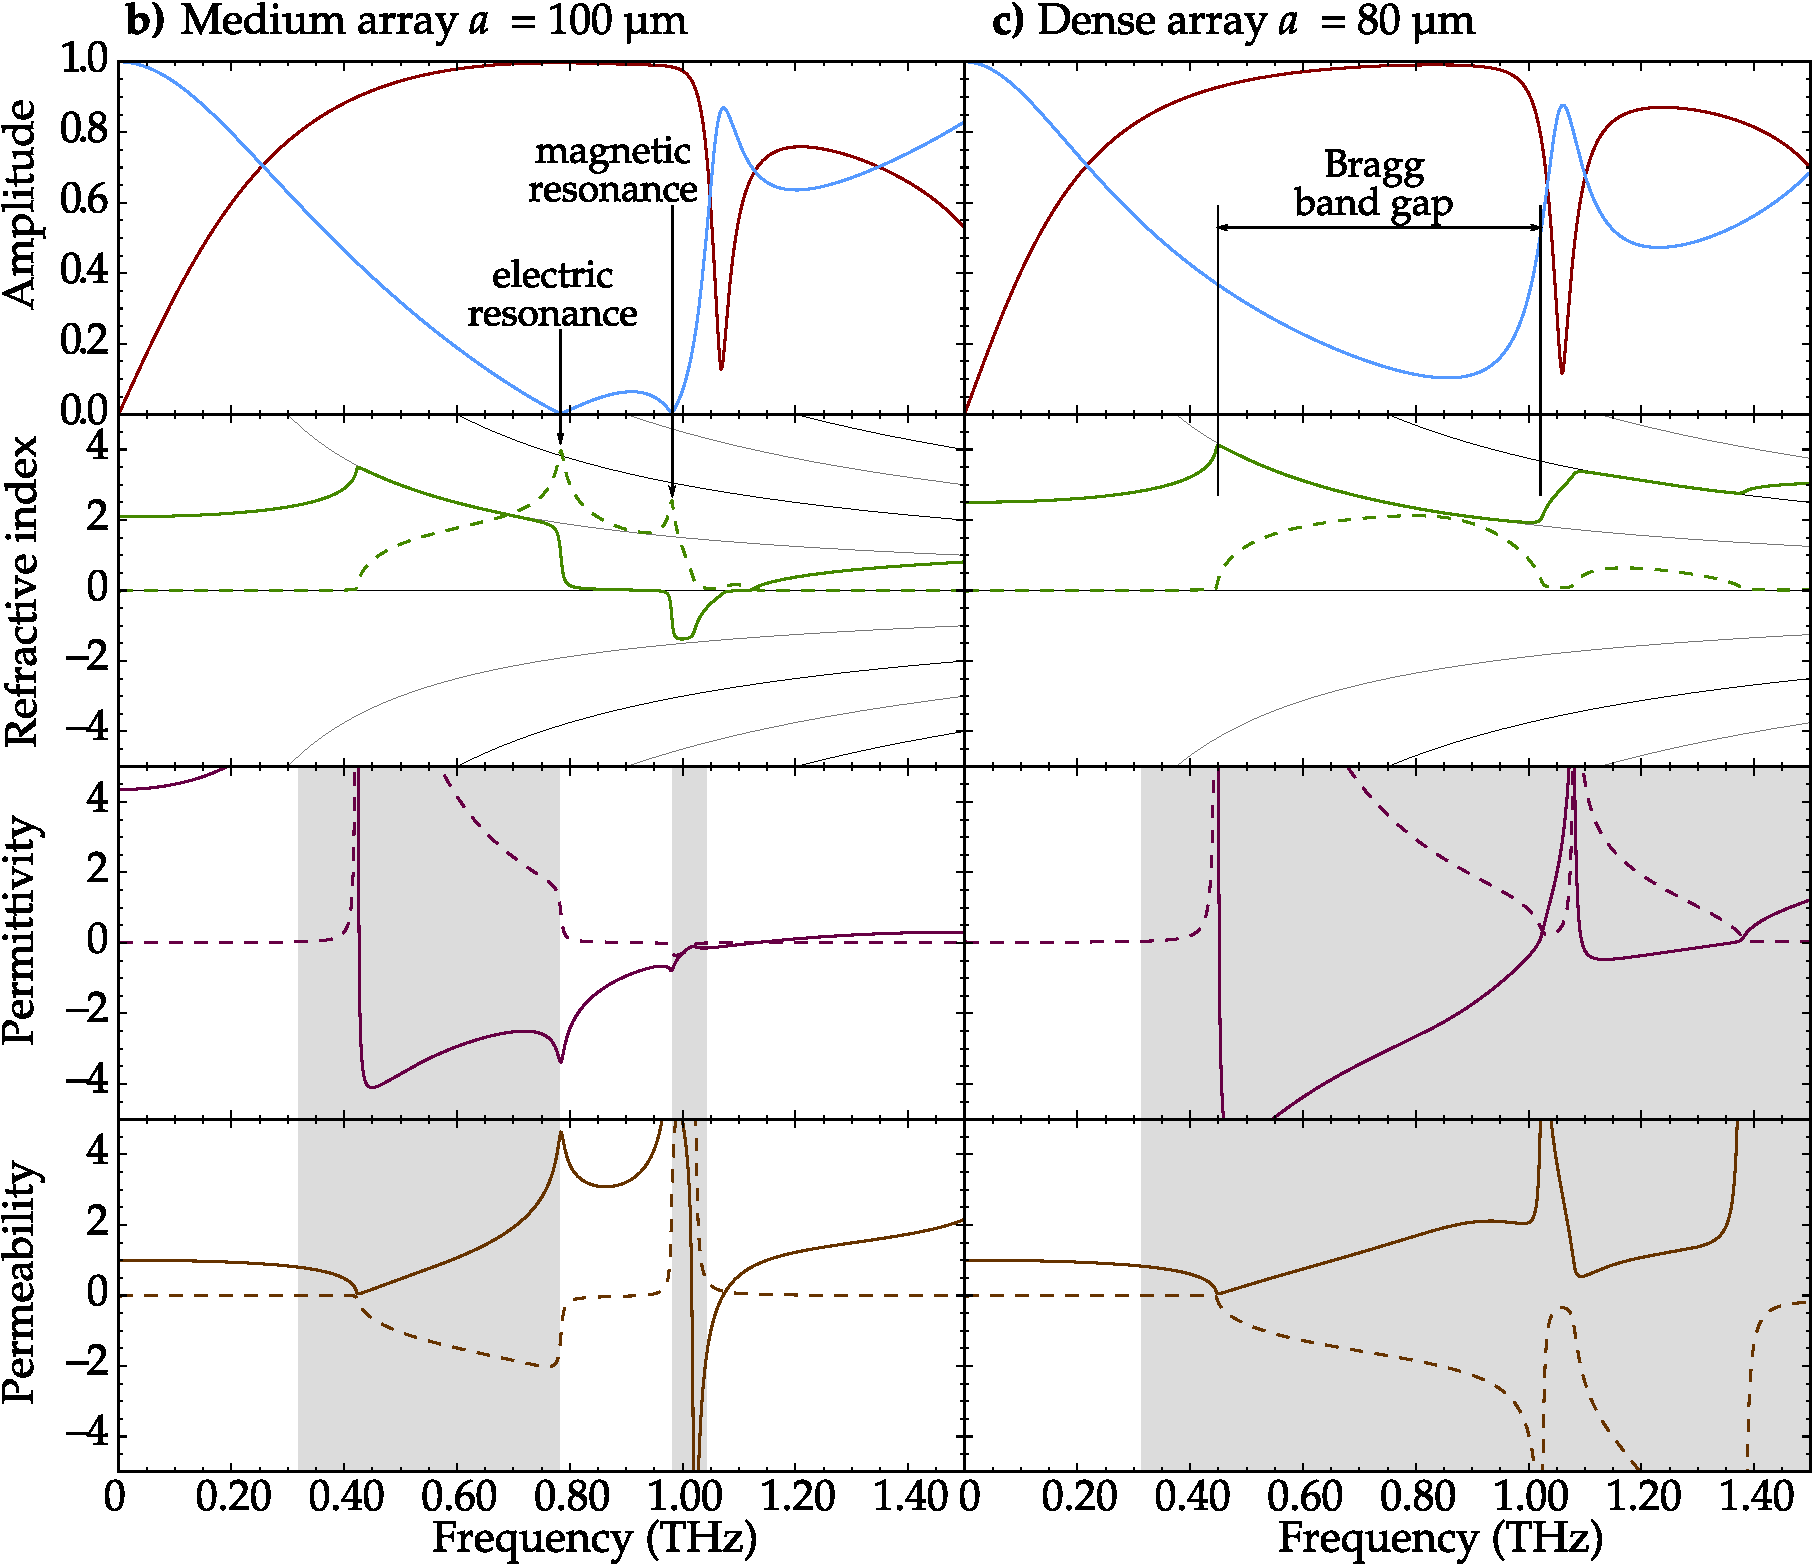
\includegraphics[width=10cm]{img/ERods_eps100_double_a100a080_FDTD.pdf} \end{figure} \clearpage


\begin{figure} \caption{img/ERods\_sketch\_of\_separate\_spectra\_to\_continuous\_scan.pdf}  \centering 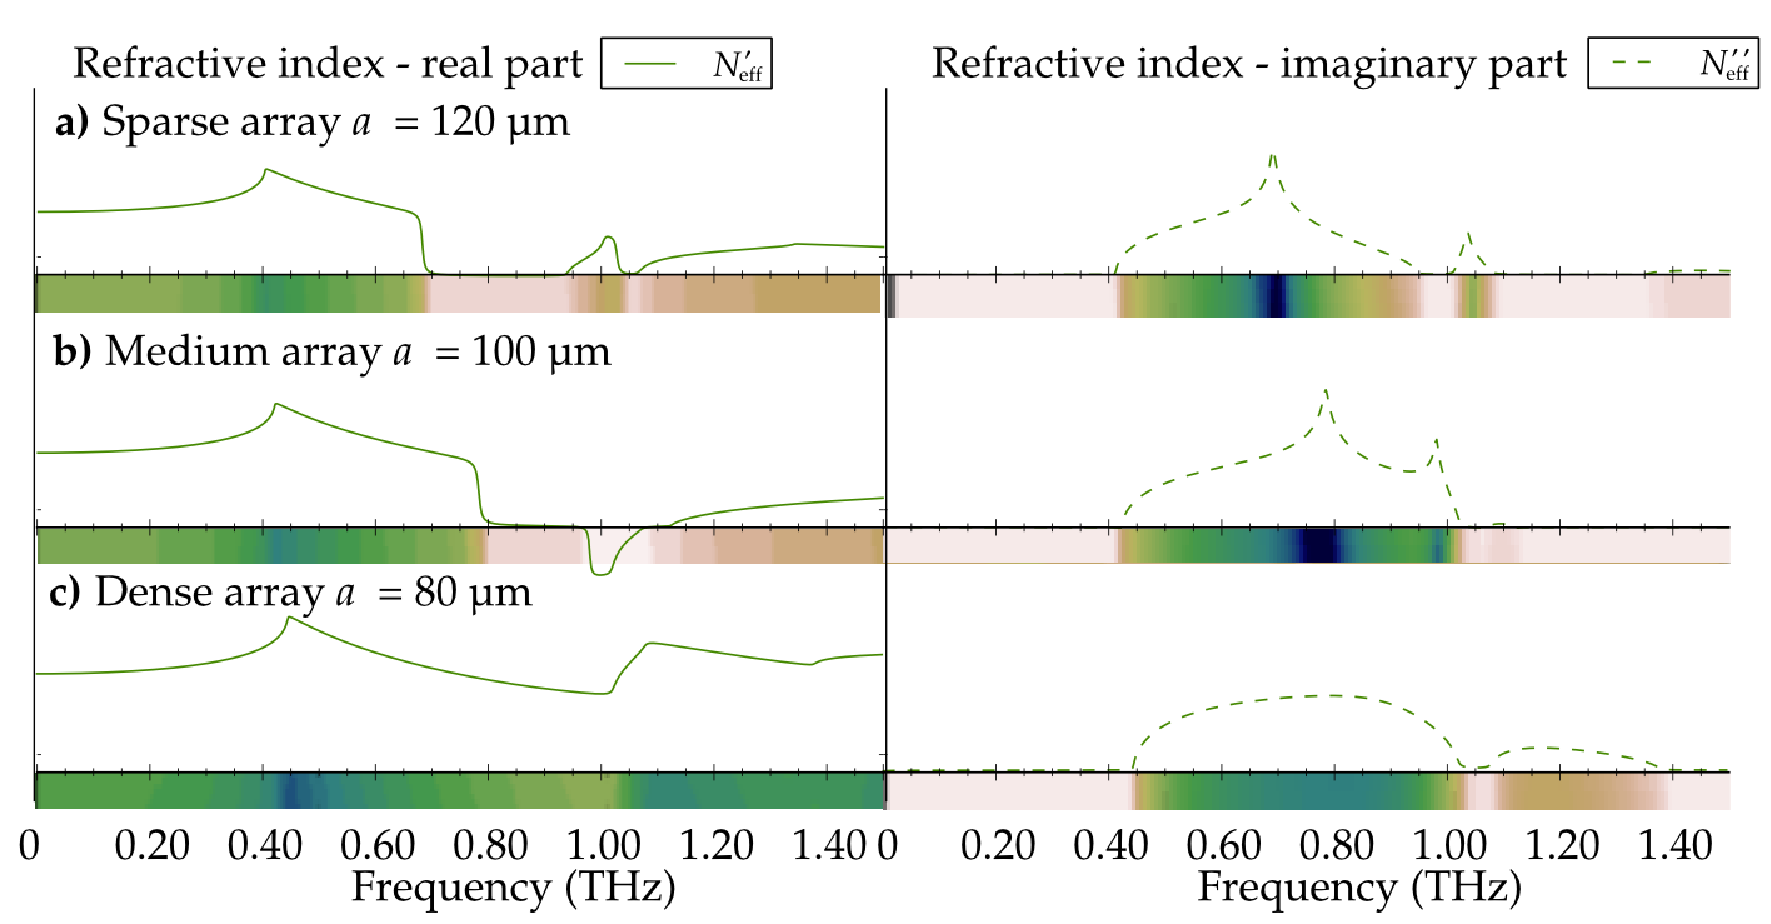
\includegraphics[width=10cm]{img/ERods_sketch_of_separate_spectra_to_continuous_scan.pdf} \end{figure} \clearpage
\begin{figure} \caption{img/ERods\_eps100\_spacingscan\_Nim.pdf}  \centering 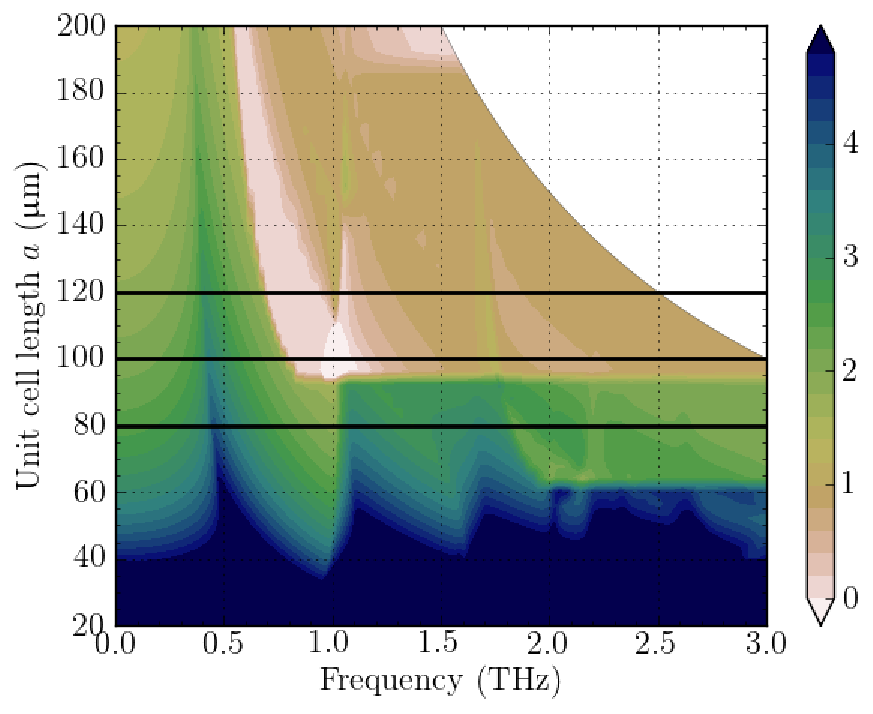
\includegraphics[width=10cm]{img/ERods_eps100_spacingscan_Nim.pdf} \end{figure} \clearpage
\begin{figure} \caption{img/ERods\_eps100\_spacingscan\_Nre.pdf}  \centering 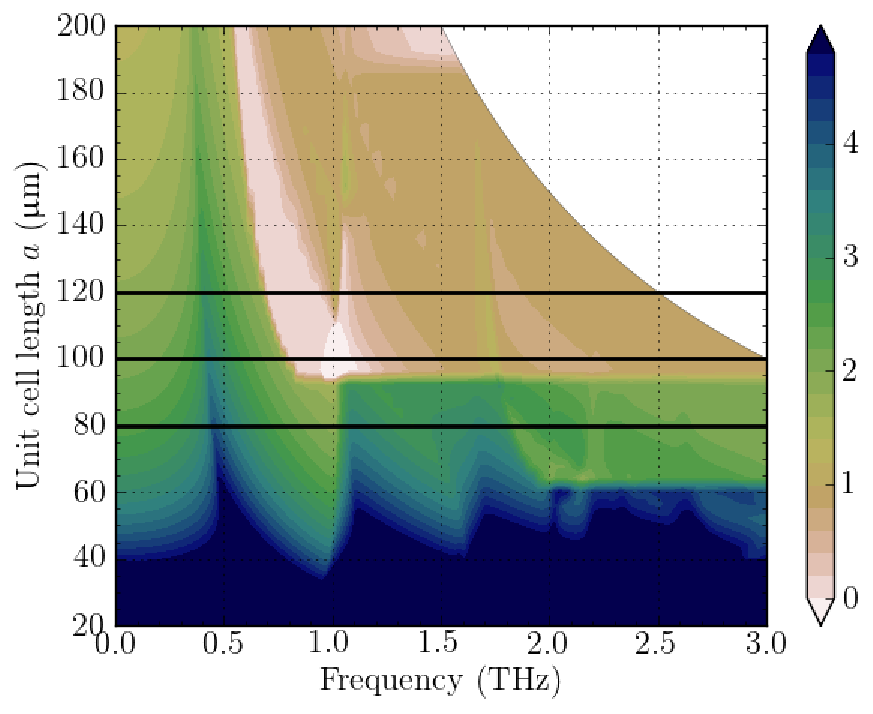
\includegraphics[width=10cm]{img/ERods_eps100_spacingscan_Nre.pdf} \end{figure} \clearpage
\begin{figure} \caption{img/ERods\_eps100\_spacingscan\_drawn\_bands.pdf}  \centering 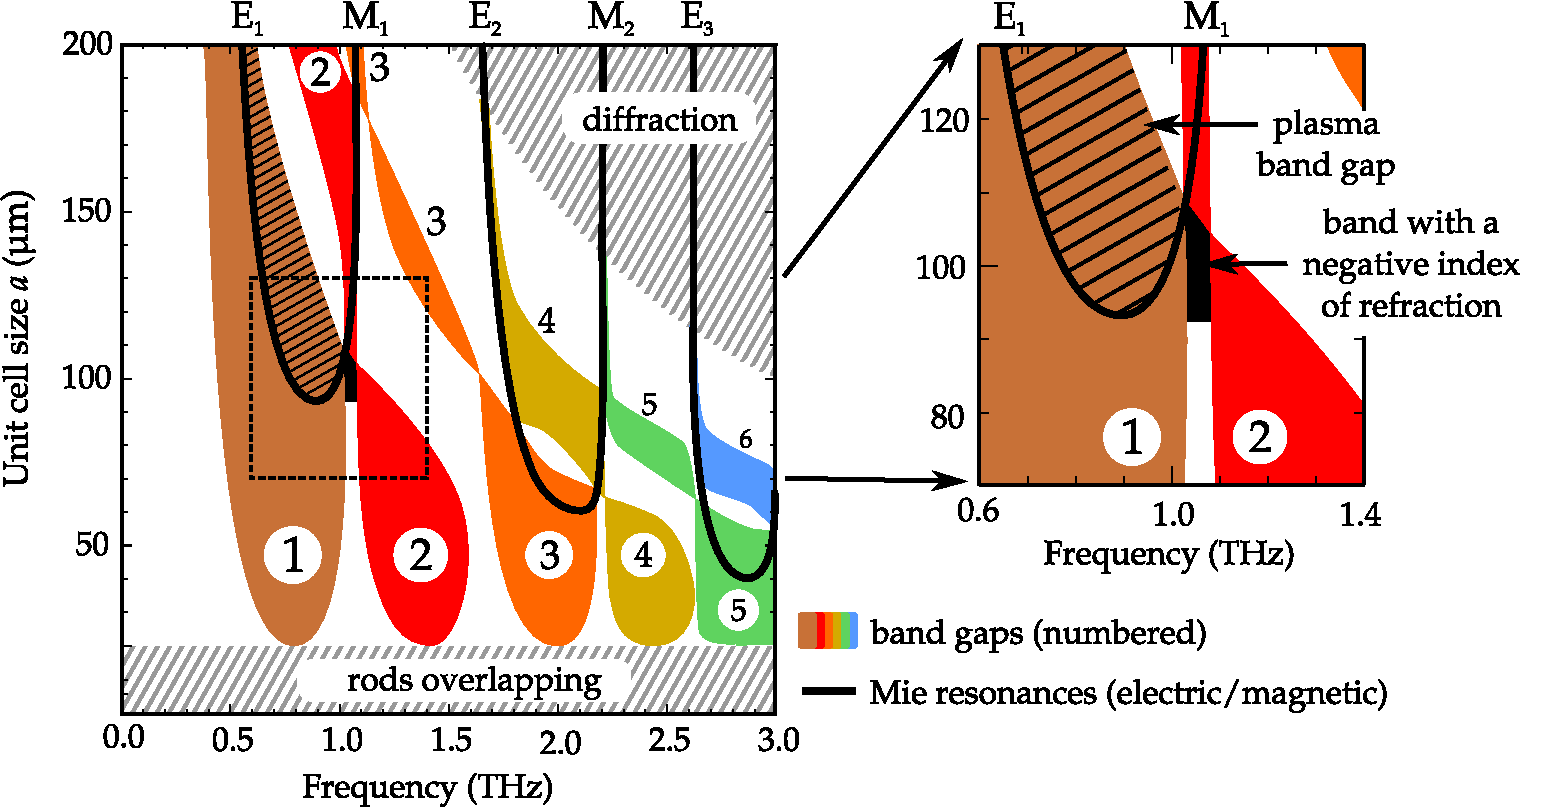
\includegraphics[width=10cm]{img/ERods_eps100_spacingscan_drawn_bands.pdf} \end{figure} \clearpage
\begin{figure} \caption{img/ERods\_eps030\_spacingscan\_drawn\_bands.pdf} \centering 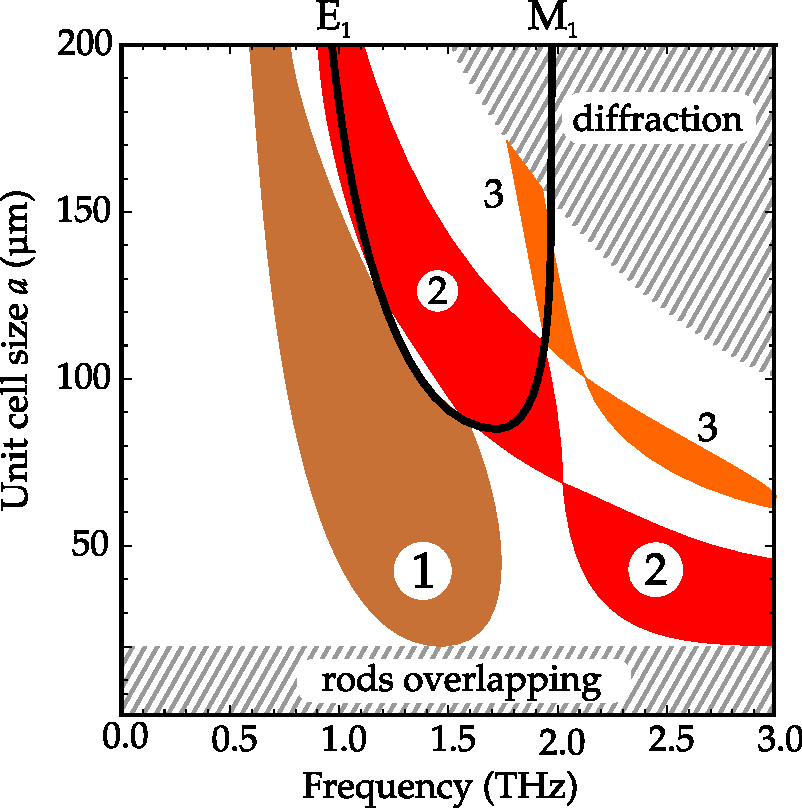
\includegraphics[width=10cm]{img/ERods_eps030_spacingscan_drawn_bands.pdf} \end{figure} \clearpage

\begin{figure} \caption{img/ERods\_eps100\_R11\_PWEM.pdf}  \centering 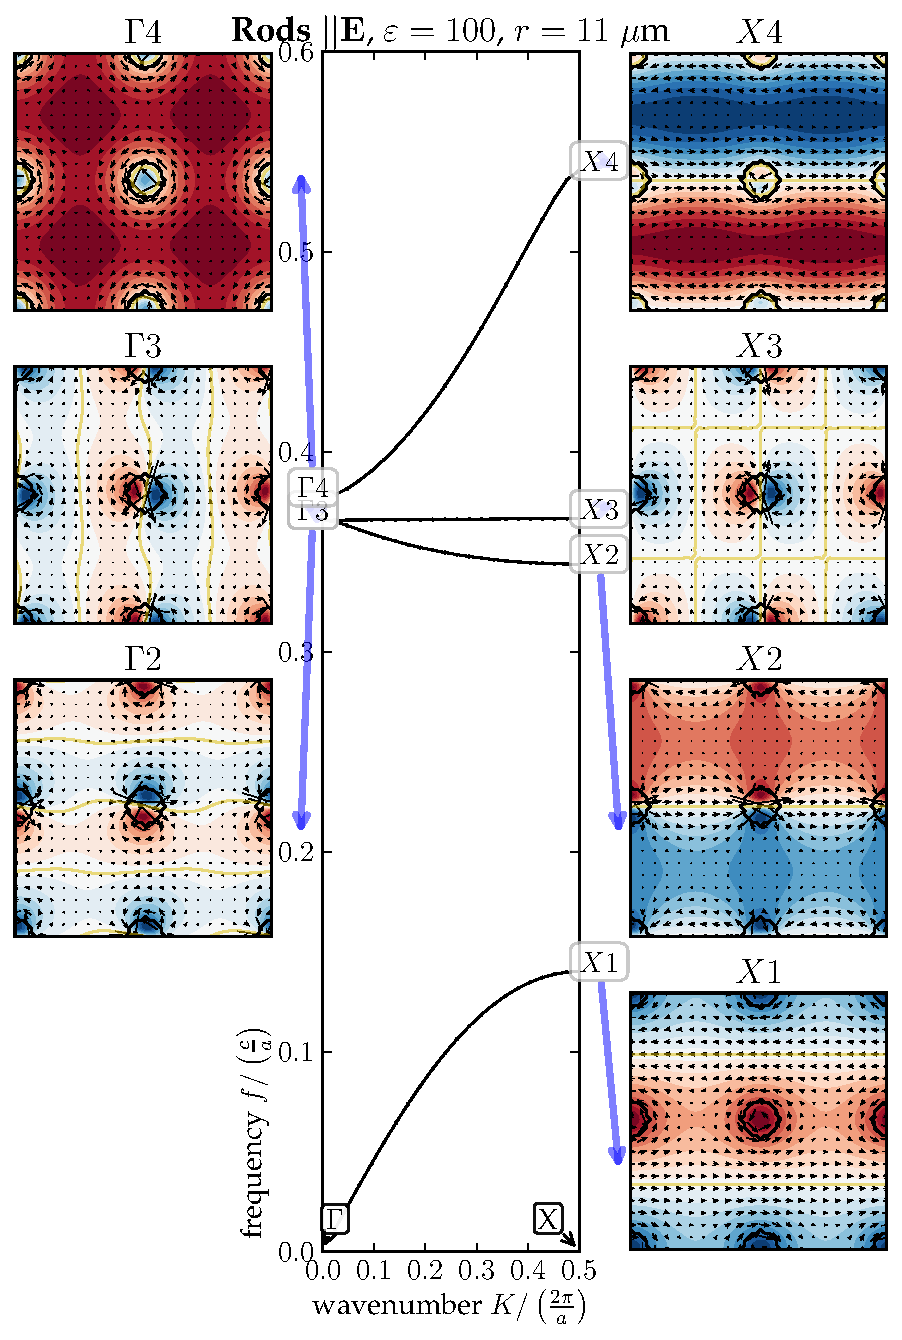
\includegraphics[width=10cm]{img/ERods_eps100_R11_PWEM.pdf} \end{figure} \clearpage
\begin{figure} \caption{img/ERods\_eps100\_single\_a120\_FDTD.pdf}  \centering 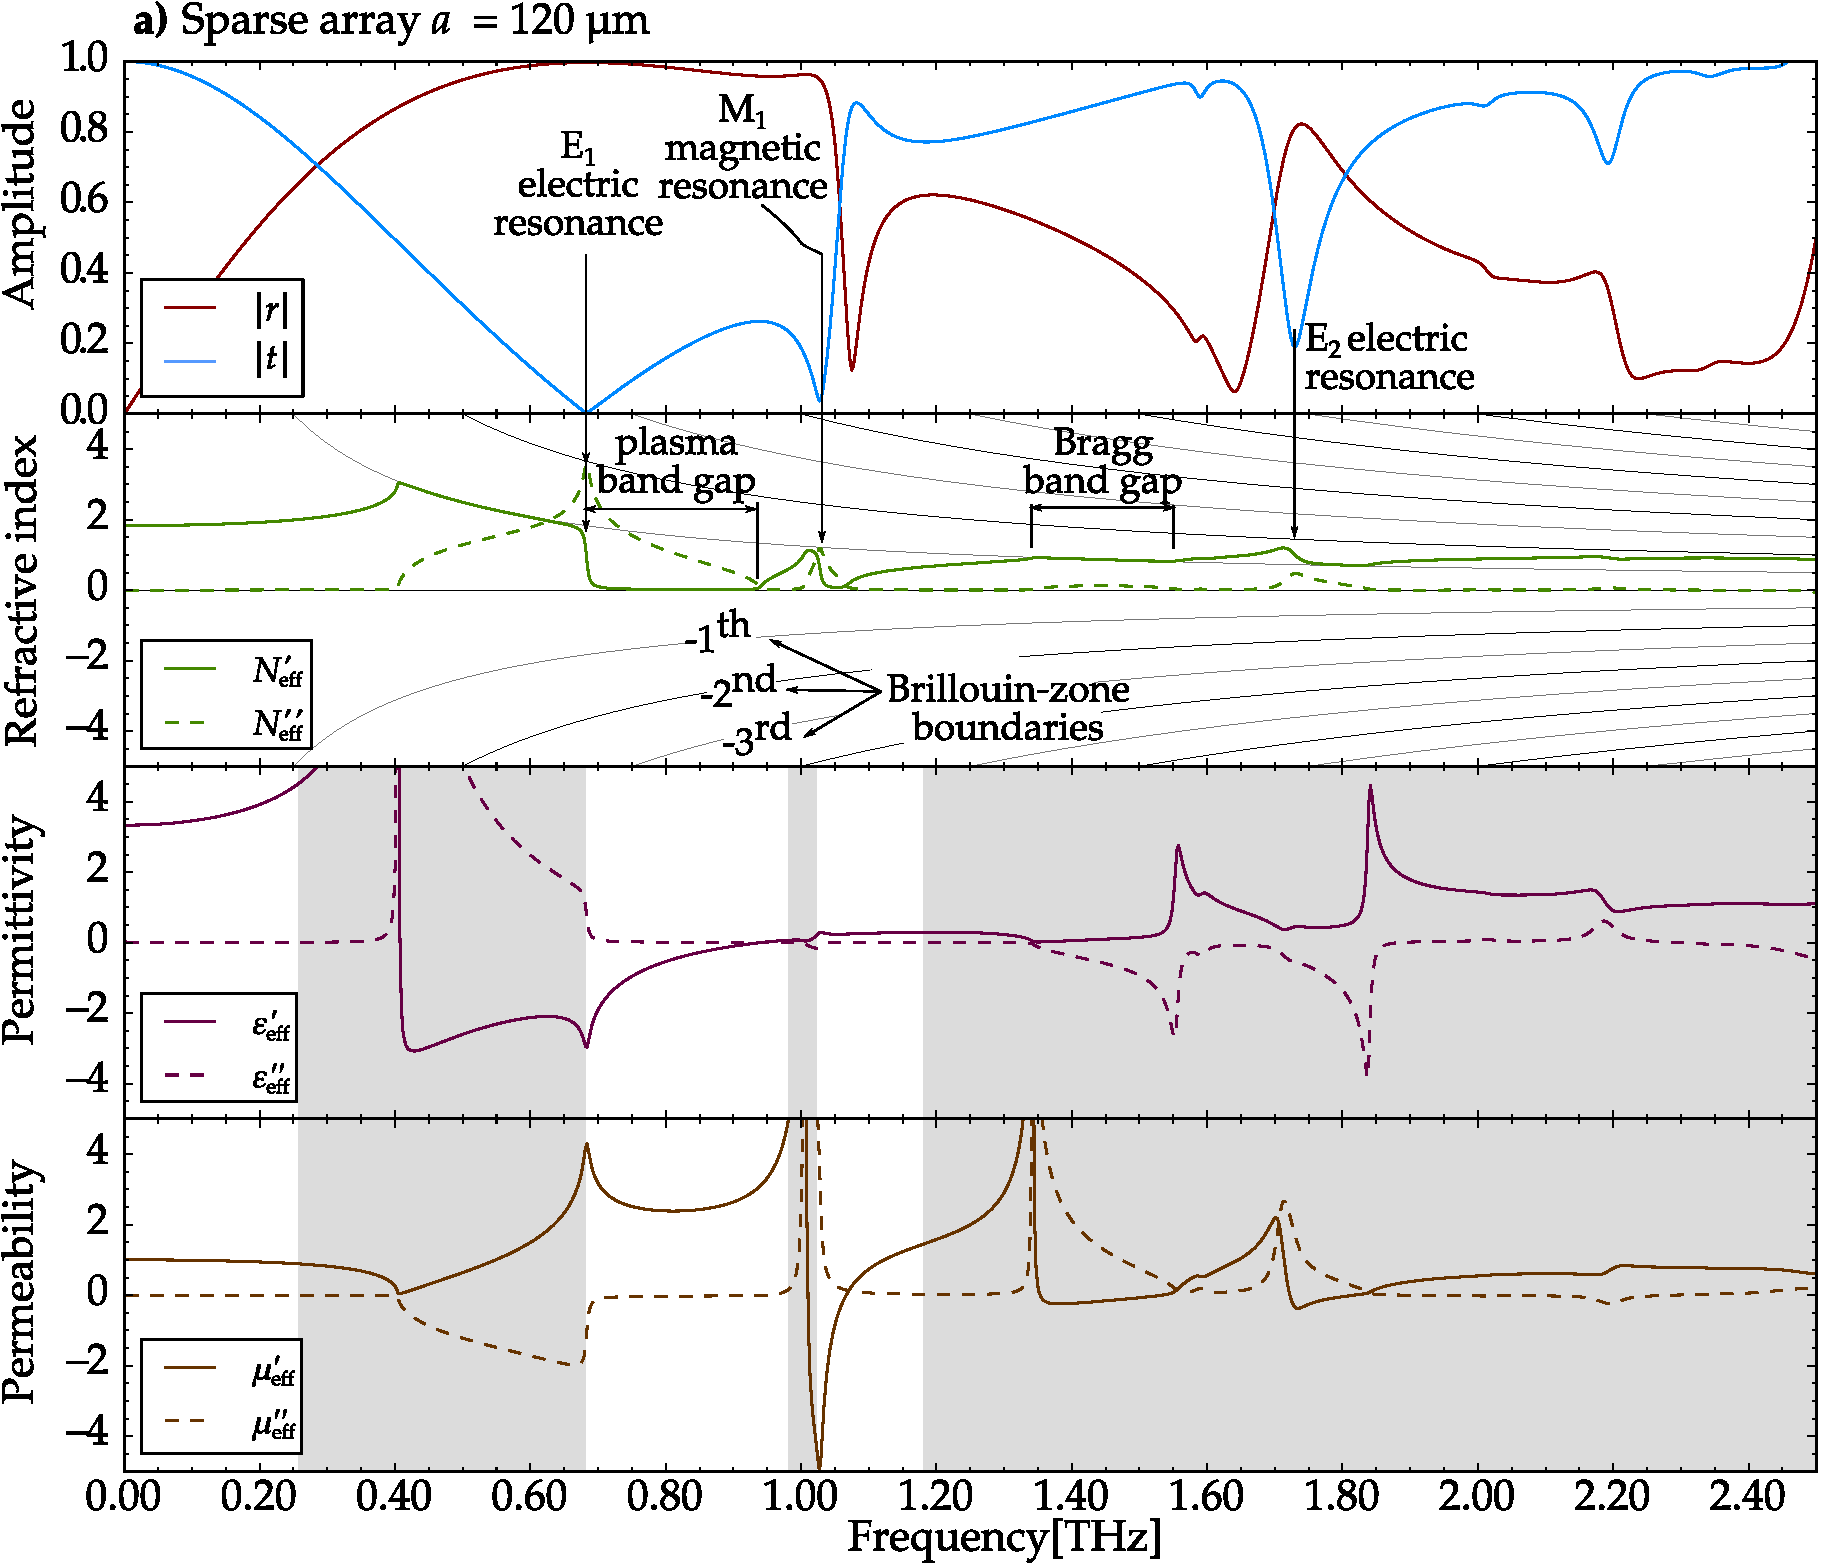
\includegraphics[width=10cm]{img/ERods_eps100_single_a120_FDTD.pdf} \end{figure} \clearpage
\begin{figure} \caption{img/ERods\_eps100\_triple\_a150a100a080\_FDTD.pdf}  \centering 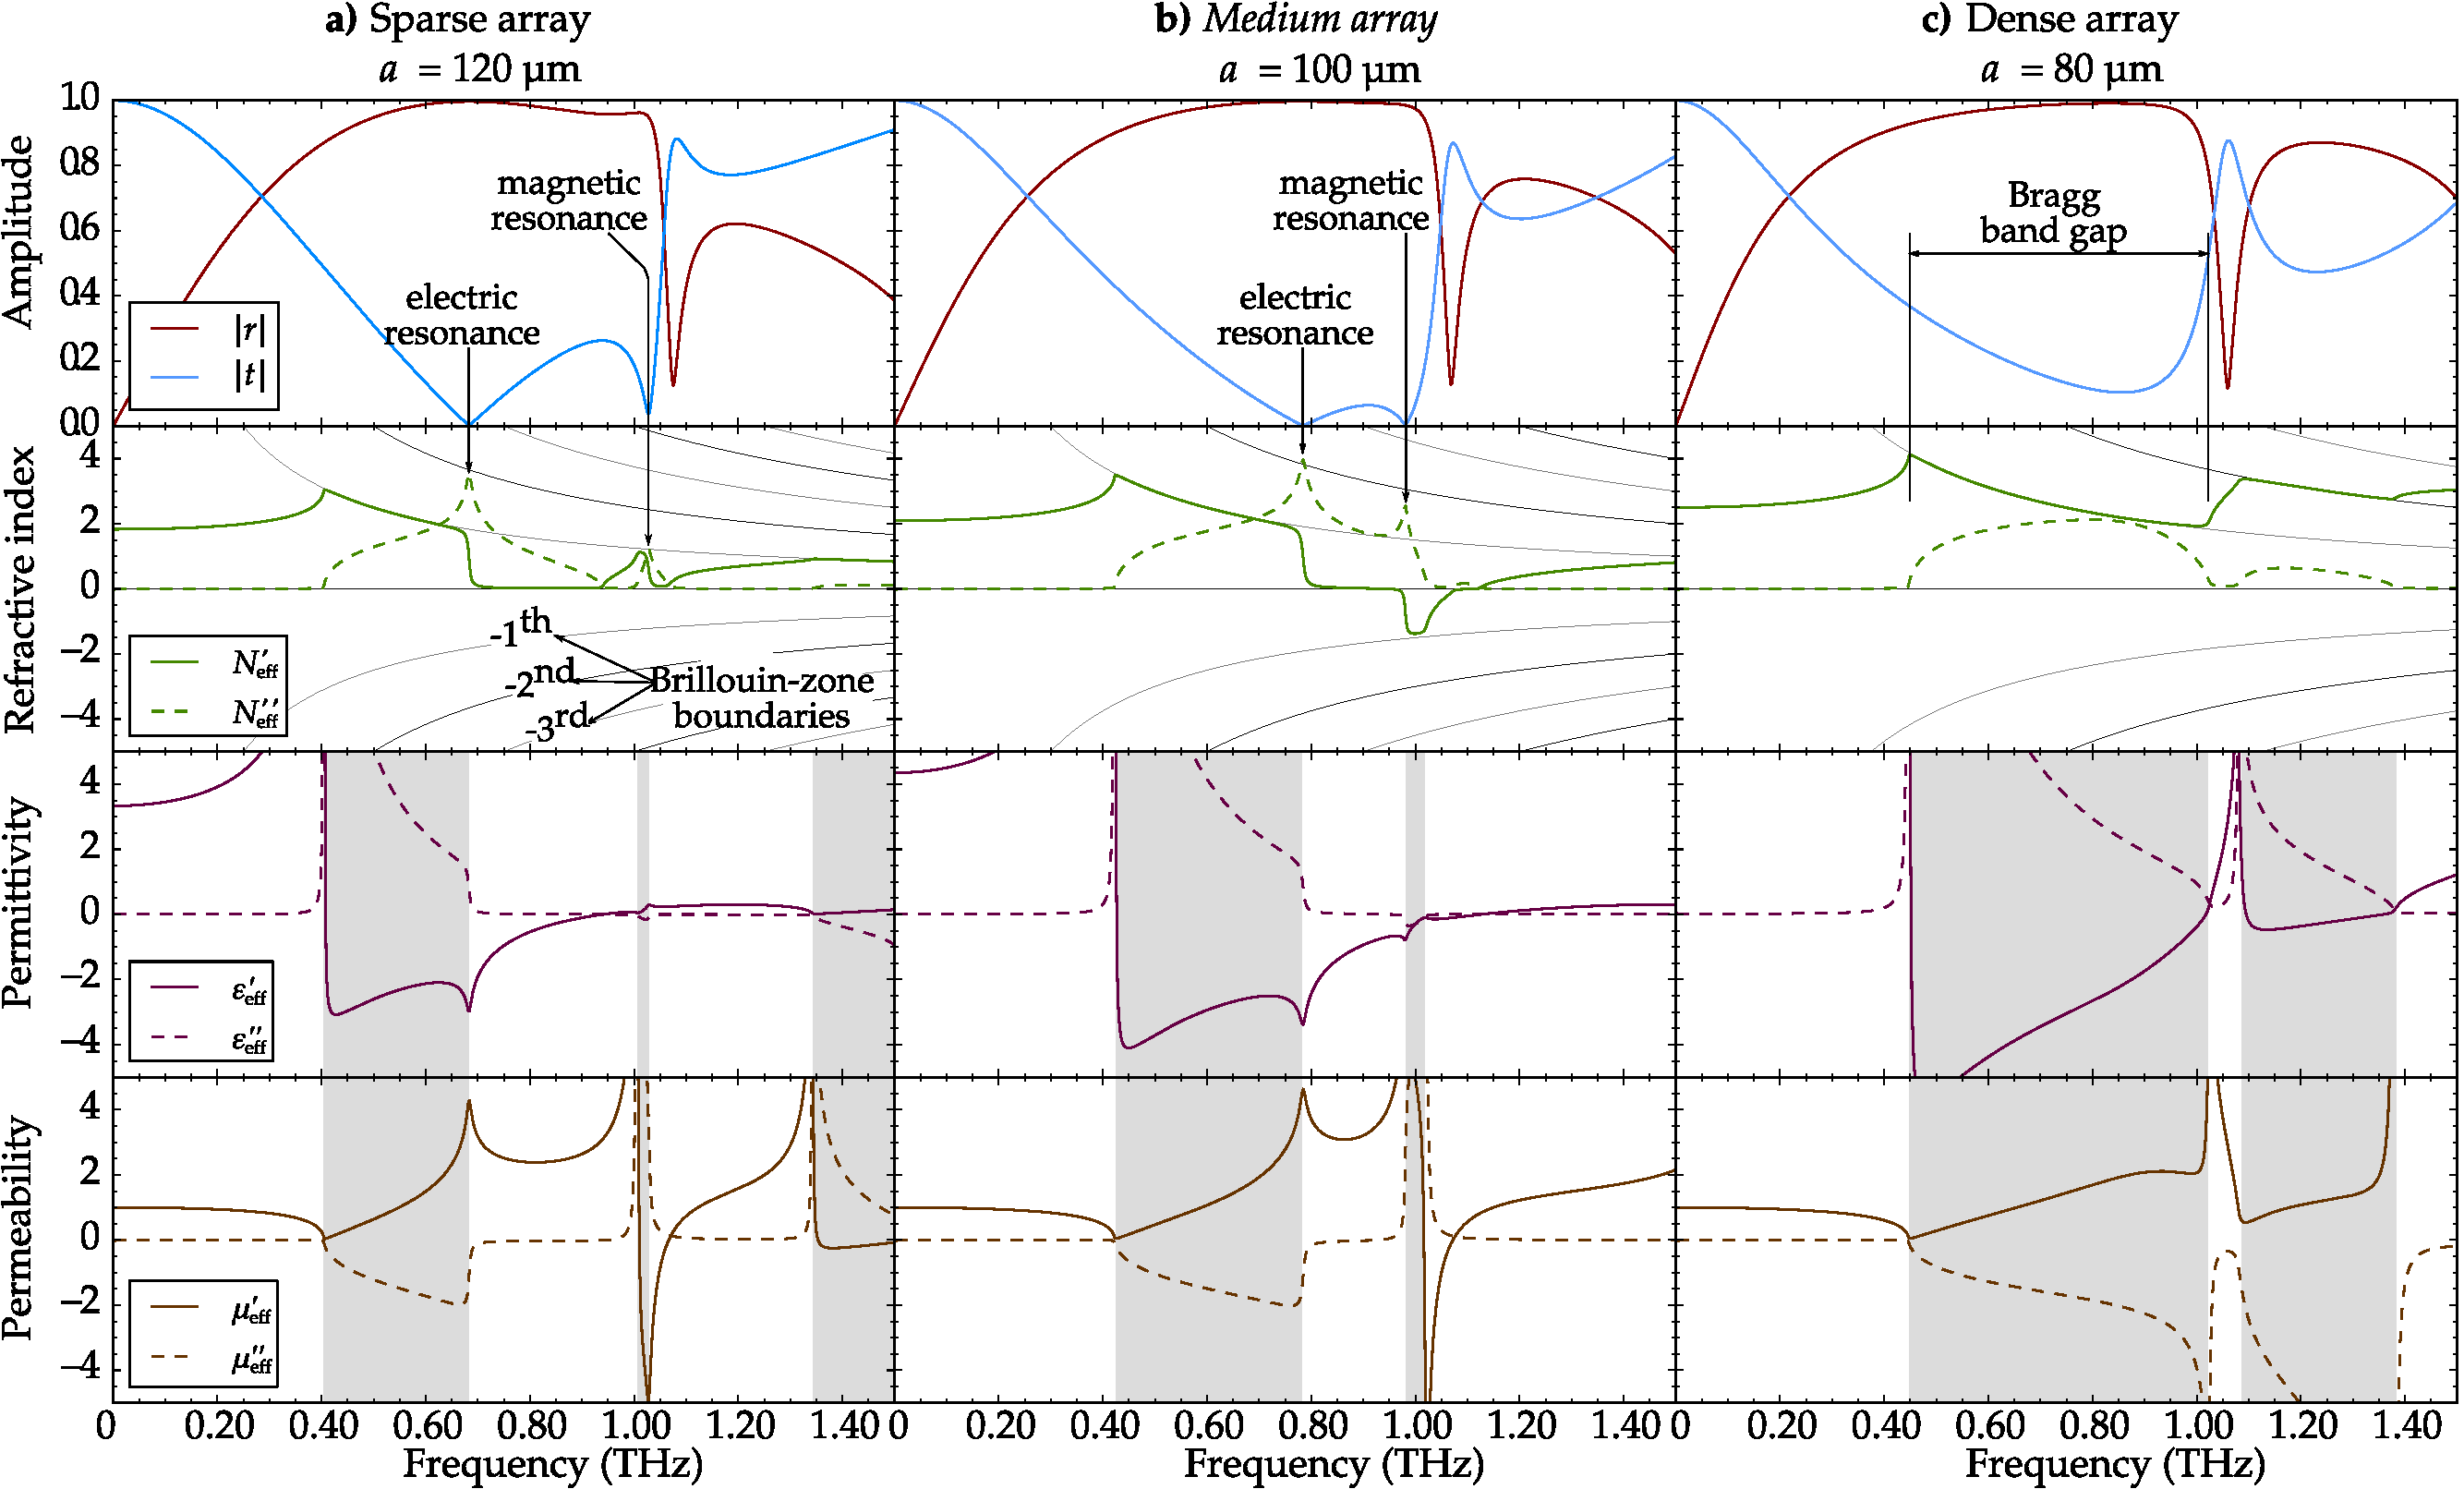
\includegraphics[width=10cm]{img/ERods_eps100_triple_a150a100a080_FDTD.pdf} \end{figure} \clearpage
\begin{figure} \caption{img/ERods\_forSeefeld\_sparserN\_denserN\_DrawnBands.pdf}  \centering 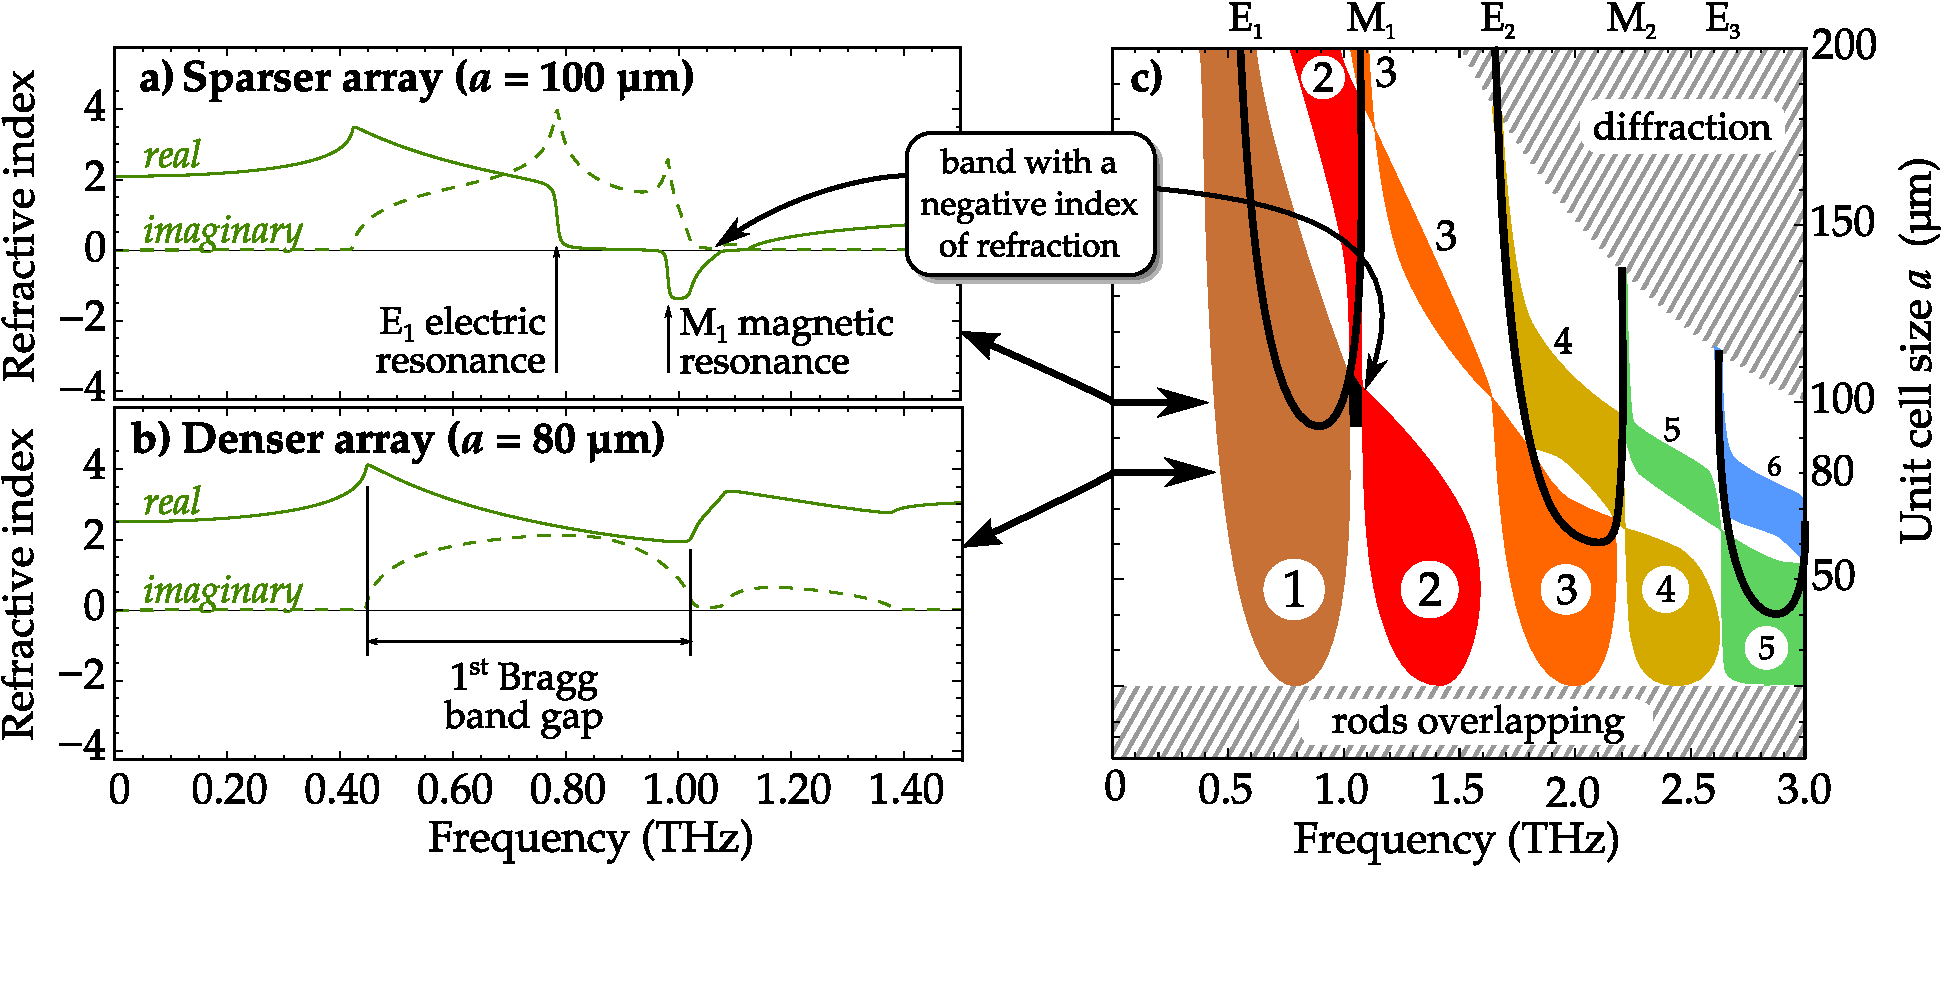
\includegraphics[width=10cm]{img/ERods_forSeefeld_sparserN_denserN_DrawnBands.pdf} \end{figure} \clearpage


\begin{figure} \caption{img/ERods\_sketch\_recordedline.pdf}  \centering  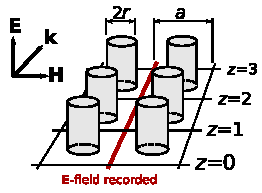
\includegraphics[width=10cm]{img/ERods_sketch_recordedline.pdf} \end{figure} \clearpage
\begin{figure} \caption{img/ERods\_eps100\_R10u5\_FXplot.pdf}  \centering 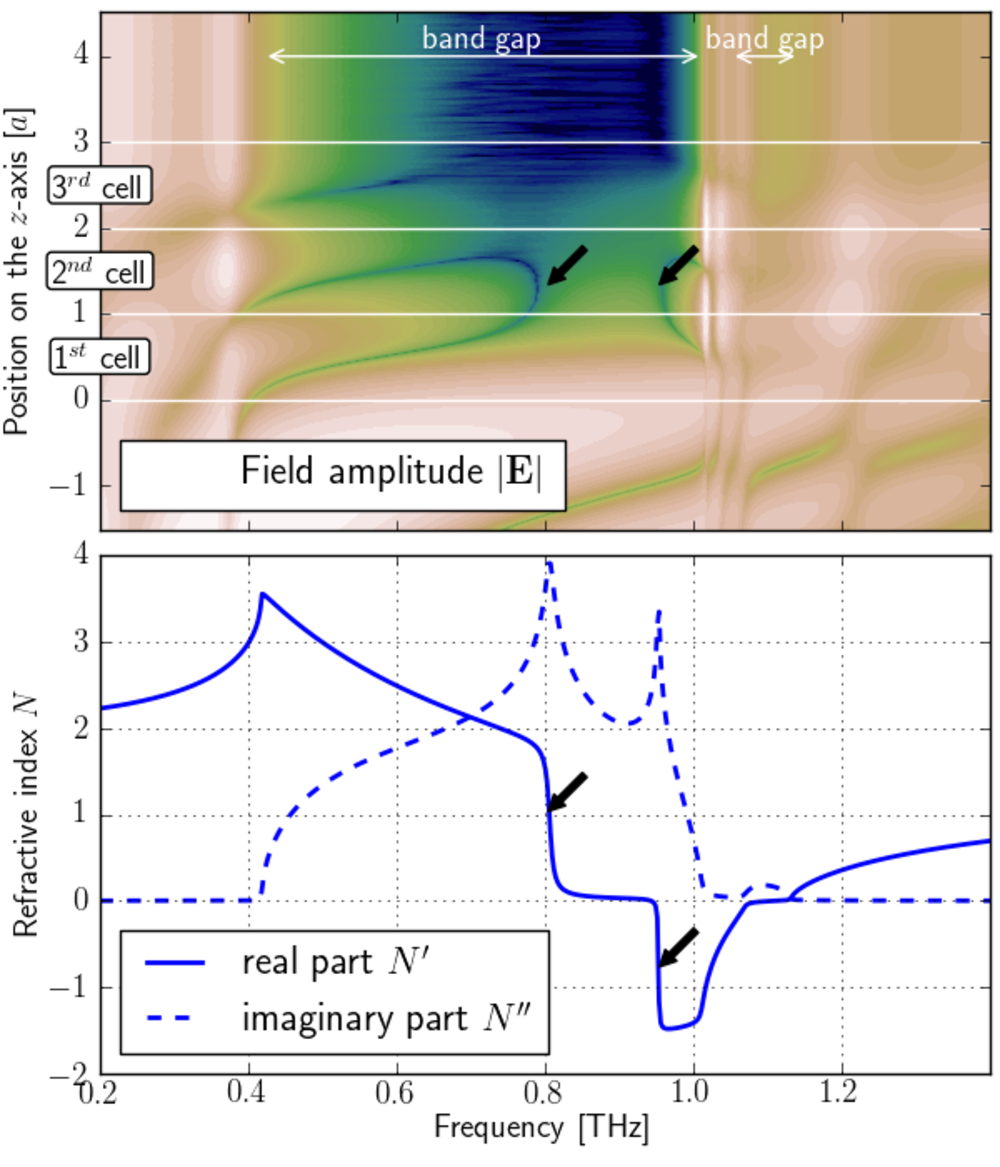
\includegraphics[width=10cm]{img/ERods_eps100_R10u5_FXplot.pdf} \end{figure} \clearpage
%}}}
\section{Metallic screen with a slit} % references to ->
\section{A fishnet - metallic screen with holes} % references to ->
%{{{
\begin{figure} \caption{img/fishnet.pdf}  \centering 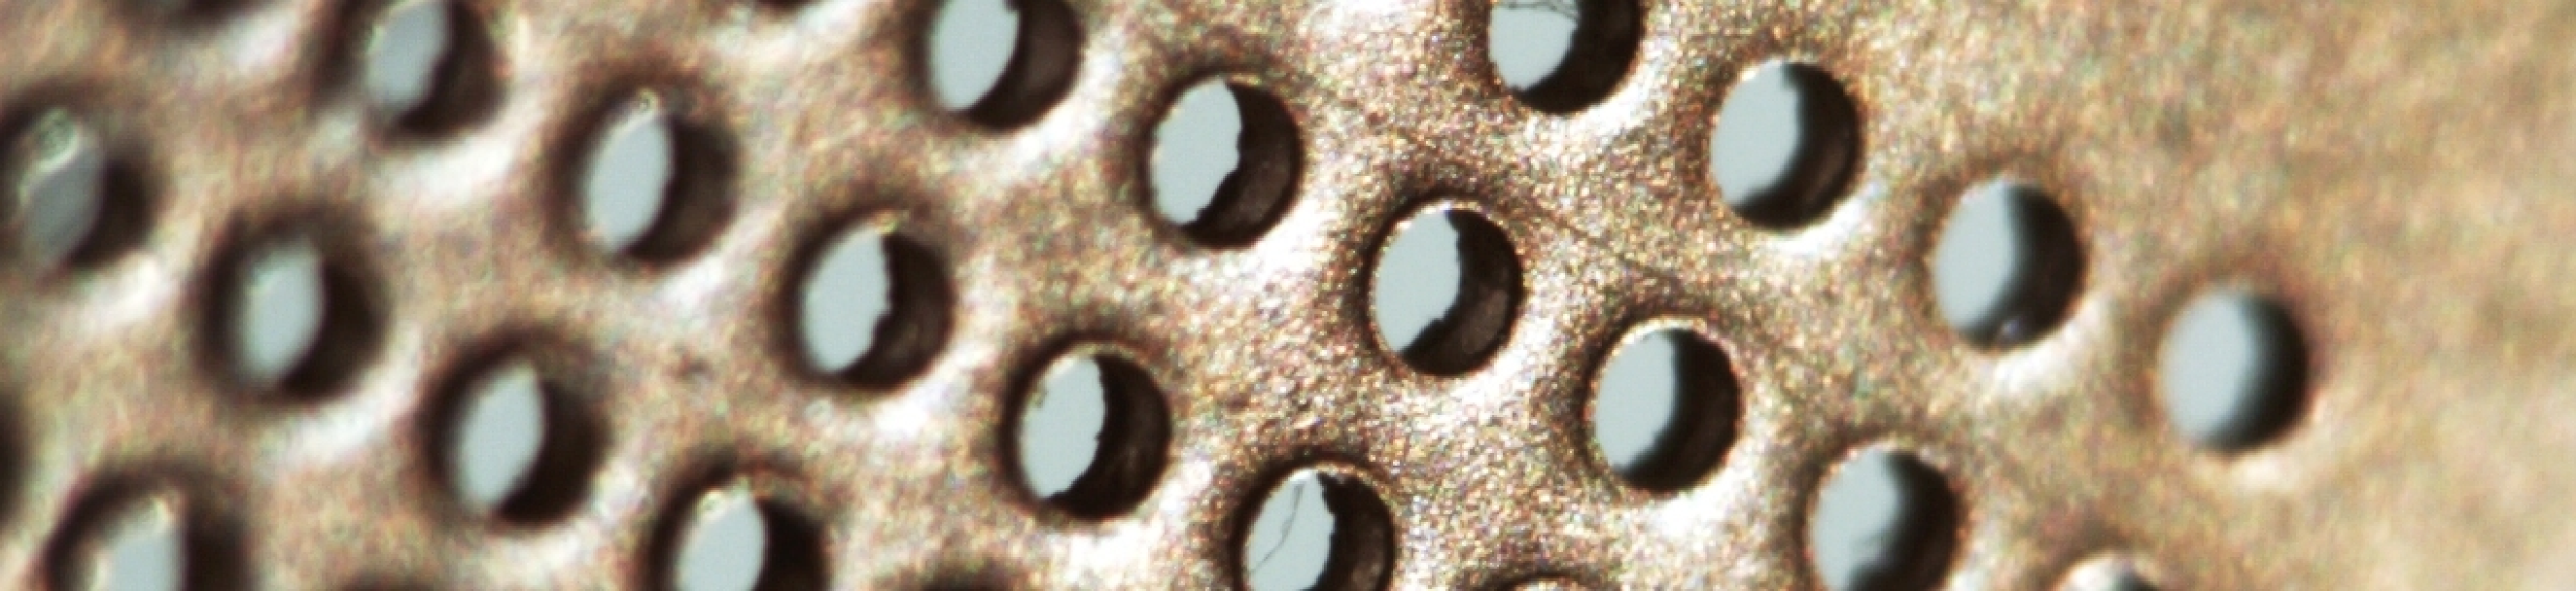
\includegraphics[width=10cm]{img/fishnet.pdf} \end{figure} \clearpage
%}}}

\section{Other structures} % plasmonic spheres (note: resonance width determined by gamma of the metal?)
\begin{figure} \caption{Modes in sphere-wire structure}  \centering 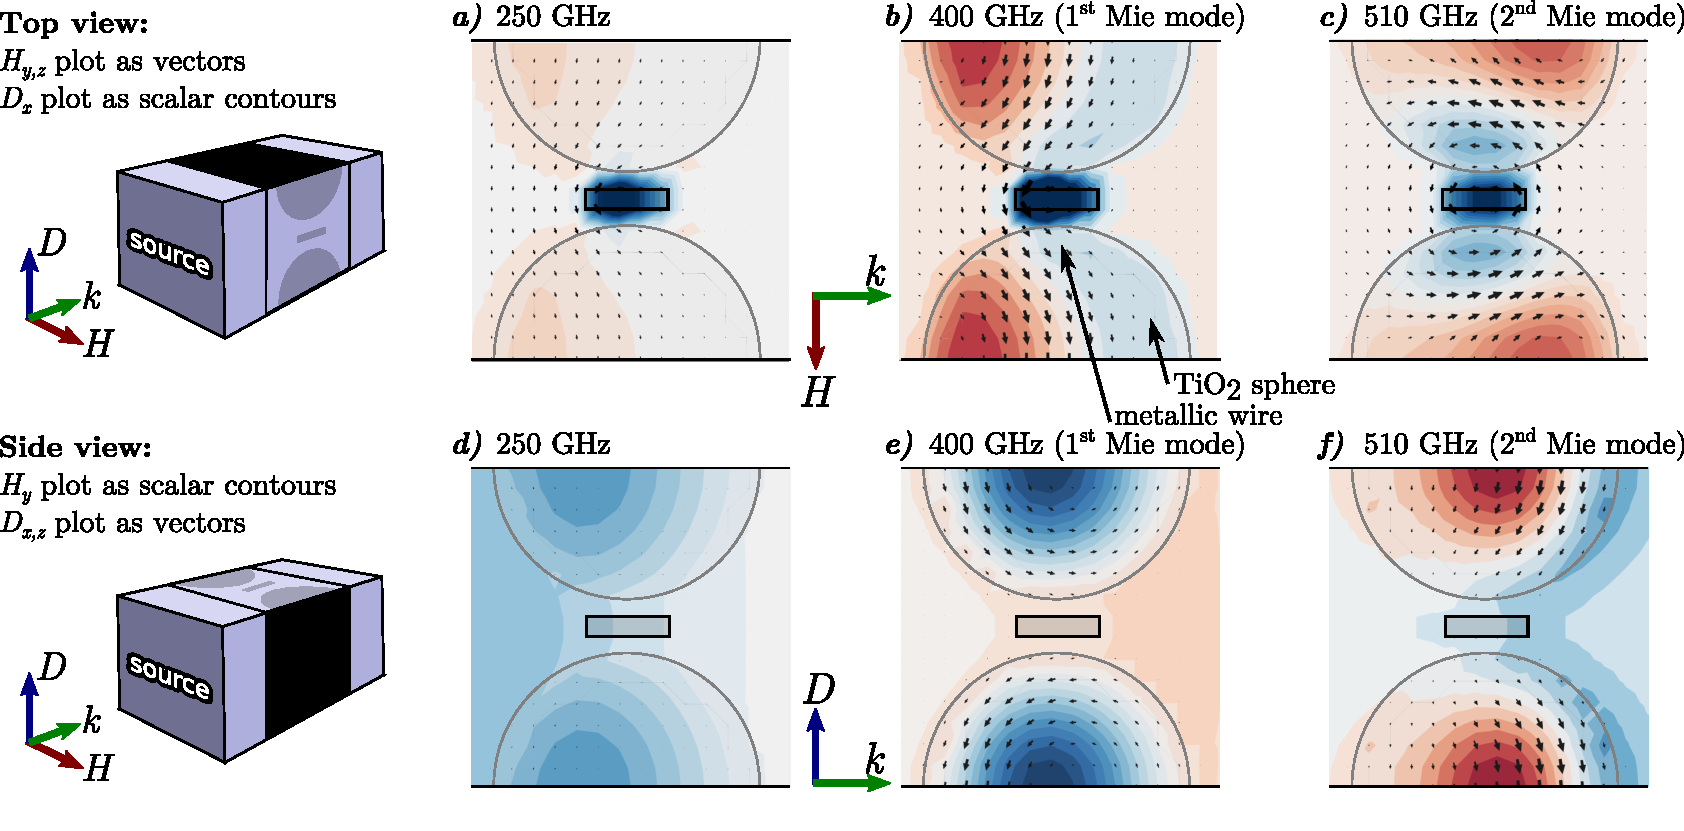
\includegraphics[width=10cm]{img/new/modes_Mag_and_El.pdf} \end{figure} \clearpage
\subsection{} % references to ->
\subsection{} % references to ->
\subsection{} % references to ->
\subsection{} % references to ->
\subsection{} % references to ->
